%!TEX program = xelatex

\documentclass[color=pdftex,usenames,dvipsnames, aspectratio=169]{beamer}
%\includeonlylecture{intro}
\usepackage{pgfpages}
%\setbeameroption{show notes on second screen}
\setbeameroption{hide notes}
\definecolor{mygray}{gray}{0.9}
\definecolor{amber}{rgb}{1.0, 0.75, 0.0}

\usepackage[english]{babel}
\usepackage[default]{lato}
\usepackage{listings}
\usepackage{fancyvrb}
\usepackage{tikz}
\usepackage{refcount}
\usepackage{gensymb}
%\usepackage{enumitem}
\usepackage{pdfoverlay}

% 
%% Colors used in the document
% \color{Apricot}
% \color{blue}
% \color{BrickRed}
% \color{OliveGreen}
% \color{orange}
% \color{purple}
% \color{RedOrange}
% \color{teal}
% \color{violet}
% \color{yellow} - highlight in title

% \usepackage{caption}
% \captionsetup[figure]{labelformat=empty}

\mode<presentation>{
\useoutertheme[numbering=counter]{metropolis}
\useinnertheme{metropolis}
\usefonttheme{metropolis}
\usecolortheme{orchid}
}
\setbeamertemplate{note page}{\pagecolor{yellow!5}\insertnote}

\hypersetup{
    colorlinks,
    linkcolor={red!50!black},
    citecolor={blue!50!black},
    urlcolor={blue!80!black}
}

% \captionsetup{labelformat=empty,labelsep=none}
%\lstset{frame=shadowbox,language=Java,basicstyle=\footnotesize}
\lstset{%
    language=Java,
    basicstyle=\ttfamily\color{blue},
    keywordstyle=\bfseries\color{black!80!white},
    commentstyle=\slshape\color{OliveGreen},
    identifierstyle=\bfseries\color{purple!50!black},
    stringstyle=\color{violet},
    escapechar=\#,
    emphstyle=\bfseries\color{red},
    showspaces=false,
    upquote=true,
    xleftmargin=0.2in,
    xrightmargin=0.1in,
    framexleftmargin=0.1in,
    backgroundcolor=\color{mygray},
    columns=fullflexible,
    literate={*}{{\char42}}1
             {-}{{\char45}}1
             {\ }{{\copyablespace}}1,
    frame=single,
    framerule=1pt,
    rulecolor=\color{OliveGreen}
}

% \setlist[itemize]{noitemsep}
% \setlist[enumerate]{noitemsep}

\usepackage[space=true]{accsupp}
\newcommand{\copyablespace}{\BeginAccSupp{method=hex,unicode,ActualText=00A0}\hphantom{x}\EndAccSupp{}}
\setlength{\parindent}{0em}

\title{Robotics - Event Driven Programming}
\author{Dave Cohen}
\institute[Comp. Sci., RHUL]{Computer Science, Royal Holloway, University of London}
\date[Term 2, 2020/2021]{Term 2, Academic Year 2020/2021}
\subject{Robotics}

\AtBeginLecture{\setcounter{framenumber}{0}\frame[standout,plain]{\insertlecture}}
\AtBeginSection{
\begingroup
\setbeamercolor{palette primary}{bg=yellow!30!white}
\frame[standout,plain]{\sectionpage}
\endgroup
}

\beamertemplatenavigationsymbolsempty 
% \fboxsep=1mm%padding thickness
% \fboxrule=1pt%border thickness
%\setbeamercovered{invisible}


\begin{document}

\begin{frame}
  \titlepage
\end{frame}

\lecture{Introduction}{intro}

% \subsection{Robot Groups and Coding the EV3}
\begin{frame}<1>[label=groups]{Groups}
\begin{block}<1-2>{Deliverables}
\begin{itemize}
\item You will work in groups of three or four.
\textbf{Everyone programs.}
\item You will give a group presentation at the end of module.\\
\textit{Not everyone has to present - you all get the same grade.}
\item You will give a public robot demonstration in the summer term.\\
\textit{Not everyone has to demonstrate - you all get the same grade.}
\item You will submit an individual report: \textbf{your own work!}.\\
\item Your grades are very strongly affected by your participation.\\
\item The five worksheets count towards your participation score.
\end{itemize}
\end{block}
\end{frame}
\begin{frame}<1>[label=twos]{Succeeding in Groups}
\begin{block}<1-2>{Worksheets and Progress}
\begin{itemize}
\item \textcolor{OliveGreen}{Worksheets help you to pace your progress (One+ per week).}
\item \textcolor{teal}{Every worksheet needs you to program the robot.} 
\item \alert{You submit the code on Moodle.}
\item \textcolor{RedOrange}{Stronger group members should run their own tutorials.}
\item Course leaders and/or tutors will be available at all sessions to help.
\item \textcolor{RedOrange}{Use the Piazza forum to ask questions}
\item \textcolor{OliveGreen}{We can help to fix robots that go bad.}
\item \textbf{Everyone codes.}
\end{itemize}
\end{block}
\end{frame}

\begin{frame}<1>[label=projects]{Projects}
\begin{block}<1-2>{Kinds of Lego Robot}
\begin{itemize}
\item \textcolor{Blue}{Brilliant} Table Toddler (maybe maps the table).
\item \textcolor{purple}{Inspired} Wall Follower (maybe maps the room).
\item \textcolor{OliveGreen}{Clever} Line Follower (maybe decides what to do at junctions).
\item \textcolor{violet}{Sublime} Object Counter (could sort objects as well).
\item \textcolor{teal}{Maze solver, Card Player, Musical Instrument player, Intelligent Cars\dots}
\item \textcolor{RedOrange}{Towers of Hanoi}, \dots, \alert{anything else agreed by me!}
\end{itemize}
\end{block}
\begin{alertblock}<1-2>{Moodle}
There is a much more extensive list on Moodle.
\end{alertblock}
\end{frame}

\begin{frame}{Many groups will use Android via Bluetooth}
\begin{block}{EV3Sensors and an Android Phone \textcolor{yellow}{Fun with Phones}}
The GitHub  account \href{https://github.com/cyclingProfessor}{cyclingProfessor} has a repository called \texttt{EV3Sensors} that will connect successfully to an EV3 brick, and can do \alert{OpenCV image processing}, \alert{find QR codes} and \alert{reads NFC tags}.

You must load it into a properly installed \texttt{Android Studio} on your own machine.
\begin{itemize}
  \item \textcolor{OliveGreen}{You can use it as a set of extra sensors for your brick.}
  \item For example \textcolor{OrangeRed}{QR, NFC}, FaceFinder and Proximity Sensor
  \item \textcolor{teal}{Or a (much) better output device than the LCD on the robot.}
\end{itemize}
\end{block}
\begin{block}{EV3Dev Examples}
\alert{The Ev3Dev-examples repository is useful: eg for the EV3Dev program for \texttt{EV3Sensors}. }
\end{block}
\end{frame}

\begin{frame}{Some Groups use the PC}
\begin{block}{Robot Code}
\alert{The same robot code can run on the PC and control the robot. !}

\textcolor{OliveGreen}{Then you have all of the Java ecosystem (and APIs).}

\textcolor{violet}{This lets you use a proper Java user interface and perhaps a map on the screen etc.,}
\end{block}
\end{frame}

\begin{frame}{Every Group uses the Behaviour design pattern}
\begin{block}{Behaviours: \textcolor{yellow}{Walking, talking, eating and falling}}
\textcolor{OliveGreen}{When we are \emph{walking} about (a low-level behaviour) we can also be \emph{eating} and \emph{talking}.}

\begin{itemize}
\item  None of these three behaviours suppresses any of the others.

\item \textcolor{teal}{The \emph{eating} behaviour uses our hands.}

\item \textcolor{violet}{The \emph{Walking} behaviour uses our legs.}

\item \textcolor{OrangeRed}{The \emph{eating} behaviour share the mouth with \emph{talking} }
\end{itemize}

\textcolor{RedOrange}{If we \emph{fall over} this will \alert{suppress} all the other three behaviours.  }
\begin{itemize}
\item \textcolor{violet}{It is a higher level behaviour.}
\end{itemize}

We can program robots using this \alert{subsumption architecture}.
\end{block}
\end{frame}

\begin{frame}{Extending Behaviours: States and Personality}
\begin{block}{Changing from one state of certainty to another}
\begin{itemize}
\item We can control the flow of behaviours using a \texttt{state} field.
\item We can make a set of behaviours active using \texttt{Personality} objects. 
\item Different personalities can share some \texttt{Behavior} objects.
\item We can even use the \texttt{state} field and behaviours to separate claps.
\item \alert{Drawing a state diagram is a very useful process.}
\end{itemize}
\end{block}
\end{frame}

% \subsection{It is easy to begin}

\begin{frame}[fragile]{Square Dancing Robot}
\begin{block}{Its So Easy:}
\begin{enumerate}
 \item Do FOUR times:
\begin{enumerate}
 \item Go Forward.
 \item Turn Left
\end{enumerate}
\end{enumerate}
\end{block}

\begin{lstlisting}[basicstyle=\ttfamily\small\color{blue}]
BaseRegulatedMotor mLeft = new EV3LargeRegulatedMotor(MotorPort.A);
BaseRegulatedMotor mRight = new EV3LargeRegulatedMotor(MotorPort.B);
mRight.forward();
for (int i = 0 ; i < 4 ; i++) { // Do FOUR times
  mLeft.forward();  // Go forwards (side i)
  Delay.msDelay(1000);
  mLeft.stop();     // Turn a corner
  Delay.msDelay(200);
}
mRight.stop();
\end{lstlisting}

\end{frame}
\begin{frame}[fragile]{Creeper program}
\begin{lstlisting}[basicstyle=\ttfamily\scriptsize\color{blue}]
BaseRegulatedMotor mL = new EV3LargeRegulatedMotor(MotorPort.A);
BaseRegulatedMotor mR = new EV3LargeRegulatedMotor(MotorPort.D);

mL.forward(); // Start the ball rolling
mR.forward();

LCD.getInstance().drawString("Its all quiet", 2,1,0);
NXTSoundSensor us = new NXTSoundSensor(SensorPort.S1);
SampleProvider sp = us.getDBAMode();
float[] samples = new float[1];
sp.fetchSample(samples, 0); // Read Ahead Paradigm
while (samples[0] < 0.5) {
  // just keep swimming....
  sp.fetchSample(samples, 0); // Read Ahead for next loop.
}
LCD.getInstance().drawString("Wow - what a noise", 2,1,0);
mL.stop();
mR.stop();
\end{lstlisting}
\end{frame}
\begin{frame}[fragile]{Lego Does Lego}
\begin{center}
\includegraphics[width=8cm,height=4.5cm]{Videos/LEGO-Car-Factory-feat.jpg}

\href{https://www.youtube.com/watch?v=VSzkiu9uhgU}{This is above and beyond}

\end{center}
\end{frame}

% \subsection{Robots}
\begin{frame}[label=robotDef]{A Robot is\ldots}
  \begin{block}{Wiki}
    There is \alert{much} discussion about which machines qualify as robots, a typical robot will have several, though not necessarily all of the following properties:
    \begin{itemize}
     \item Is \alert{not 'natural'} i.e. has been artificially created.
     \item Can \alert{sense} its environment.
     \item Can \alert{manipulate things} in its environment.
     \item Has some \alert{degree of intelligence}, or ability to make choices based on the environment, or automatic control.
     \item Is \alert{programmable}.
     \item Can make \alert{dexterous coordinated movements}.
     \item Appears to have \alert{intent} or agency
    \end{itemize}
  \end{block}
%\hyperlink{peopleQuest<1>}{\beamerreturnbutton{}}

\end{frame}

\begin{frame}{Is this a robot?}
\begin{center}
\includegraphics[width=7cm]{Images/hello-kitty-toaster.jpg}
\end{center}
\end{frame}

\begin{frame}{Is this a robot?}
\begin{center}
\includegraphics[width=0.6\textwidth]{Images/predator.jpg}
\end{center}
\end{frame}


\begin{frame}{Robot versus Remote Control}
\begin{itemize}
\item \textcolor{OliveGreen}{Robot:} has some control over itself
\item \textcolor{OrangeRed}{Remote controlled machine:} all decisions made by human operator
\end{itemize}

\begin{center}
\includegraphics[height=5cm]{Images/stanley.jpg}
\end{center}
\end{frame}


\begin{frame}{A Robot is\ldots}
\begin{block}{The International Standard Organisation defines a \emph{robot} (ISO 8373) as:
}

\begin{quote}
    An \textbf{\textcolor{OliveGreen}{automatically controlled}, \textcolor{violet}{reprogrammable}, \textcolor{teal}{multi-purpose}, \textcolor{OrangeRed}{manipulator} \textcolor{OliveGreen}{programmable}} in three or more axes, which may be either fixed in place or mobile for use in industrial automation applications.
\end{quote}
\end{block}

\begin{block}{But, how do \textcolor{yellow}{we recognise a robot}}
    Joseph Engelberger, a pioneer in industrial robotics, once remarked:
\begin{quote}
    \textcolor{RedOrange}{I can't define a robot, but I know one when I see one.}
\end{quote}
\end{block}
\end{frame}

\begin{frame}[fragile]{Robots in Sci-Fi, and beyond}
\begin{center}
\only<1>{\includegraphics[width=6cm]{Images/c3po.jpg}}
\only<2 | handout:0>{\includegraphics[width=6cm]{Images/CommanderData.jpg}}
\only<3 | handout:0>{\includegraphics[width=9cm]{Images/ex-machina-eva.jpg}}

\only<4 | handout:0>{
{\includegraphics[width=8cm,height=4.5cm]{Videos/Spot.png}}

\href{https://youtu.be/kHBcVlqpvZ8}{Just Wow - but is it a robot?}
}
\end{center}
\end{frame}
\begin{frame}[label=peopleQuest]{Are people Robots?}
\begin{block}{Are we Robots? \textcolor{yellow}{Another Definition}}
    \begin{itemize}
     \item A robot is \alert{not 'natural'} and appears to have \alert{intent} or agency
     \item Can \alert{sense} and \alert{manipulate things} in its environment.
     \item Has some \alert{degree of intelligence}: makes choices and/or \alert{runs autonomously}.
     \item Is \alert{programmable}.
     \item Can make \alert{dexterous coordinated movements}.
    \end{itemize}
\end{block}

\uncover<2>{
\begin{block}{People aren't Robots}
\begin{center}
\large
\textcolor{OliveGreen}{We aren't artificial.}

\textcolor{RedOrange}{We aren't very good at most tasks.}
\end{center}
\end{block}}
\end{frame}

\begin{frame}{Senses and Sensors}

\begin{block}{\textcolor{yellow}{A sense is} a source of information about the external world: \textcolor{yellow}{an input}.}

\begin{itemize}
\item \textcolor{OliveGreen}{You have all been taught to name the (five) human senses.}
\item \textcolor{violet}{What (extra) senses do other animals have?}
\item \textcolor{OrangeRed}{What senses can a robot have beyond these animal senses?}
\end{itemize}
\end{block}

\begin{alertblock}{Standing up}
How come, when you are standing, you don't (normally) fall over?

\end{alertblock}

\uncover<2>{
\begin{block}{Hard senses to build into a robot - involving many sensors and much processing}
\alert{Equilibrioception} is balance or acceleration: Sensor in cavities in the inner ear.

\alert{Proprioception} is body awareness: Sensors in every joint and muscle.
\end{block}}
\end{frame}


% \subsection{The EV3}
\begin{frame}<1>[label=EV3]{LEGO EV3\texttrademark}
\begin{columns}<1-2>[T]
\begin{column}{0.5\textwidth}
\begin{block}{}
LEGO Mindstorms EV3 is a programmable robotics kit released by LEGO in late August 2013.
\end{block}
\end{column}
\begin{column}{0.5\textwidth}
\begin{figure}
\includegraphics[width=\textwidth]{Images/EV3-Guy.jpeg}
\caption{A walking LEGO robot}
\end{figure}
\end{column}
\end{columns}
\end{frame}

\begin{frame}<1>[label=whyEV3]{Why LEGO EV3}

\begin{block}<1-2>{We study \textcolor{yellow}{computer science} not \textcolor{OrangeRed}{engineering}}

\begin{itemize}
\item \textcolor{OliveGreen}{The mechanical side is simple.}
\item \textcolor{violet}{It is (relatively) cheap, safe and flexible.}
\item \alert{We can program it using Java.}
\item We can build great robots.
\end{itemize}
\end{block}
\end{frame}

\begin{frame}<1>[label=EV3Brick]{The EV3 brick!}

\begin{block}<1-2>{The brains of the outfit: the EV3 computer brick}
\begin{itemize}
    \item A \textcolor{OliveGreen}{32-bit ARM9 300MHz main processor}
    \item 256 KB flash memory (For the operating system)
    \item \alert{64 MB RAM (For your program!)}
    \item \textcolor{teal}{178*128 pixel grayscale LCD} (Nice, but small)
    \item \textcolor{OliveGreen}{A single USB 2.0 port and Bluetooth} (Communicating, downloading programs etc)
    \item \alert{Four input ports} (For four I2C, UART or Analogue sensors)
    \item \alert{Four output ports} (For four Servo motors)
    \item \textcolor{teal}{A speaker} (Play sound files at sampling rates up to 16 kHz)
    \item MicroSDHC slot (used for booting EV3Dev, and saving results)
\end{itemize}
\end{block}
\end{frame}

\begin{frame}<1>[label=EV3Kit]{What we give you to play with at RHUL in your robotics kit}
\vspace*{-3mm}
\begin{columns}<1-2>[T]
\begin{column}{0.6\textwidth}
\begin{block}{Motors and Sensors}
\begin{itemize}
\item \alert{Four (servo) motors} with rotation sensors.
\item \alert{*One touch sensor.} Just a switch really!
\item \alert{One colour sensor}  with a built in red LED.
\item \alert{One NXT sound sensor.}
\item \alert{One ultrasonic sensor} for distances.
\item \alert{*One gyroscope sensor} for rotational speed.
.
\item \textcolor{OliveGreen}{*Some extra Lego pieces.}
\item \textcolor{teal}{A Lego EV3 robot brain.}
\item \textcolor{teal}{A rechargeable battery charger}
\item \textcolor{RedOrange}{Some Wires  to connect Motors and Sensors}
\end{itemize}
\end{block}
\end{column}
\begin{column}{0.4\textwidth}
\begin{figure}
\includegraphics[scale=0.18]{Images/sensors.jpg}
\caption{An EV3 brick and sensors}
\end{figure}
\end{column}
\end{columns}
\vspace*{-3.5mm}
{\let\thefootnote\relax\footnote{({\color{RedOrange}*}) We do not supply the gyroscope or touch sensors and Lego pieces until needed.}}
\end{frame}


%\end{document}


%%%%%%%%%%%%%%%%%%%%%%%%%%%%%%%%%%%%%%%
% End of introdcutory Lecture.
%%%%%%%%%%%%%%%%%%%%%%%%%%%%%%%%%%%%
\lecture{Getting Started}{LectureOne}

%\section{This Course}
\begin{frame}{Aims of the Programming Lab Robotics Project }
\begin{block}{\textcolor{yellow}{We teach Robot Programming because:}}
\begin{itemize}
\item It is fun to see programming in action.
\item By building and programming robots students will see why: \\
\textcolor{purple}{Accurate programming is important}: It hard to debug a failing robot.
\item By programming embedded systems students will see why:\\
\textcolor{OliveGreen}{Advanced programming constructs are useful.}: Robot programs are complicated.
\end{itemize}
\end{block}
\pause
\begin{block}{\dots plus}
\begin{itemize}
\item \textcolor{teal}{Creativity} --- making cool stuff
\item \textcolor{teal}{Problem Solving} --- this is a hands-off course
\end{itemize}
\end{block}
\end{frame}

\begin{frame}{Objectives of the Programming Lab Robotics Project}
\begin{block}{\textcolor{yellow}{At the end of this course students will:}}
\begin{itemize}
\item Know how to \alert{use the Eclipse IDE} to write and compile Java programs.
\item Know how to \alert{control LEGO EV3 robots} using simple EV3Dev programs.
\item Understand the use of \alert{loops, decisions and threads for robot control}.
\end{itemize}
\end{block}
\end{frame}

\begin{frame}{Course Requirements}
\begin{block}{Videos}
\begin{itemize}
\item Watch some video lectures (fun and interesting) about Lego EV3 Robotics.
\item Do five worksheets (\textbf{with deadlines}: assessed by TAs in group meetings).
\end{itemize}
\end{block}

\begin{block}{Robotics Lab}
\begin{itemize}
\item Do a \alert{group project} on robotics.
\item Write a \textcolor{violet}{final individual project report.}
\item Do a \textcolor{OrangeRed}{group presentation of your project.}
\item \textcolor{OliveGreen}{Make a Demo Video of your robot for the public.}
\end{itemize}
\end{block}
\end{frame}

\begin{frame}{Logistics of Group Work in COVID times}

\begin{block}{The \textcolor{yellow}{Robot Holder} is key to the group}
\begin{itemize}
  \item One group member needs to have the \textcolor{OliveGreen}{Basic Robbie} robot.
  \item \textcolor{OliveGreen}{Robbie} comes with a rechargeable battery and mains charger.
  \item This \textcolor{purple}{Robot Holder} has certain responsibilities.
  \item The \textcolor{purple}{Robot Holder} runs code from all the group members.
  \item \dots and shows the group what is happening on zoom/teams/discord\dots
  \item You can change \textcolor{purple}{Robot Holder} - but do it COVID safely.
  \item \alert{Keep Checking Moodle, Piazza and your email}
  \item Keep the robot charged up.
\end{itemize}
\end{block}
\end{frame}

\againframe<2>{twos}
\againframe<2>{EV3}
\againframe<2>{whyEV3}
\againframe<2>{EV3Brick}
\againframe<2>{EV3Kit}
\againframe<2>{projects}

\begin{frame}[fragile]{A Lego robot that reads a Sodoku, Solves it and writes in the answer.}
\begin{center}
\href{https://www.youtube.com/watch?v=coKi3SRw_Dk}{\XeTeXLinkBox{\includegraphics[width=8cm,height=4.5cm]{Videos/Sodoku.png}}}
\end{center}

\begin{block}{Basic questions to ask when you see a new robot}
\begin{itemize}
\item \textcolor{OliveGreen}{How many effectors} does this robot have (that change the world)?
\item \textcolor{RedOrange}{How many sensors} does this robot have (that notice the world)?
\item \textcolor{purple}{How could I improve this robot?}
\end{itemize}
\end{block}
\end{frame}

\section{A Robot Design Exercise}


\begin{frame}{Robot Design - \alert{Learning by doing} - You will need a sheet of A4 paper}
\vspace*{-3mm}\centering{\Large \textcolor{OliveGreen}{If you’re watching a video - pause it now}}

\begin{block}{\textcolor{yellow}{Design a robot} that tries to stay 30cm from the wall on its left.}

\begin{itemize}
  \item Draw a rectangular robot.
\item  \textcolor{teal}{Your robot should have} \alert{distance sensors} and \alert{motors}. 
\item Show the positions, names (and directions) of the sensors and motors. 
\end{itemize}
\end{block}

\begin{block}{Write a short \alert{structured English description} of the \textcolor{yellow}{\Verb!main!} method.}

\begin{itemize}
\item \textcolor{teal}{Send messages to motors} to make them turn.
\item \textcolor{teal}{Send questions to the distance sensors} to ask them their value.
\item \textcolor{purple}{Use a WHILE loop, variables and IF statements.}
\end{itemize}
\begin{centering}
\end{centering}
\end{block}

 \textbf{Can your robot begin anywhere is the room and find a wall?}

\vspace*{-2mm}\textbf{\alert{What does the robot do when it hits unexpected corners?}}


%TODO
\end{frame}

\begin{frame}[fragile=singleslide]{A (first) solution}
\begin{lstlisting}[linewidth=12cm,emph={THEN, DO,OD,IF,FI}]
TURN L_Motor ON
TURN R_Motor ON
DO FOREVER // An infinite while loop
  IF front_distance < 30 THEN
    TURN 90 degrees RIGHT // using L_Motor and R_Motor
  FI
OD
\end{lstlisting}

\vspace*{-1.7cm}\begin{center}\includegraphics[width=5cm]{Images/bitmap.png}\end{center}
\end{frame}

\begin{frame}[fragile=singleslide]{A (second) solution}
\begin{lstlisting}[linewidth=14cm,emph={DO,OD,IF,FI,WHILE,ELIHW}]
WHILE battery level > 7v DO
  IF left distance < 25 TURN wheels RIGHT a bit.
  IF left_distance > 25 AND left_distance < 35 POINT STRAIGHT
  IF front_distance < 30 TURN RIGHT maximum.
  IF left_distance > 35 TURN wheels LEFT a bit.
ELIHW
\end{lstlisting}

\vspace*{-1.25cm}\begin{center}\includegraphics[width=5cm]{Images/bitmapLeft.png}\end{center}
\end{frame}

\begin{frame}[fragile=singleslide]{A (nother) solution}
\vspace*{-2mm}
\begin{lstlisting}[basicstyle=\ttfamily\scriptsize\color{blue}, linewidth=10cm,emph={CALL,DO,OD,IF,FI,WHILE,ELIHW,THEN}]
WHILE battery level > 7v DO
  CALL KEEP_LEFT
  IF CALL AVOID CRASH says "its safe" THEN
    speed up a bit (bounded by MAX_SPEED)
  FI
ELIHW
\end{lstlisting}
\vspace*{-3mm}
\begin{columns}[T]
\begin{column}{0.4\textwidth}
\begin{lstlisting}[basicstyle=\ttfamily\scriptsize\color{blue}, linewidth=6.5cm,emph={PROC,AS}]
PROC KEEP_LEFT
  Get left_distance AS left_one
  Wait until 1/10 sec passed.
  Get left_distance AS left_two
  Get angle from left_one and left_two
  Adjust turn to compensate.
\end{lstlisting}
\end{column}
\begin{column}{0.55\textwidth}
\begin{lstlisting}[basicstyle=\ttfamily\scriptsize\color{blue}, linewidth=7.7cm,emph={CALL,DO,OD,IF,FI,WHILE,ELIHW,THEN}]
PROC AVOID_CRASH // Return true if no wall seen
  IF front_distance < 100 THEN
    slow down a fair amount (but do not stop)
    IF front_distance < 30 THEN
      STOP
      WHILE front_distance < 80
        Turn right 5 degrees on spot.
      ELIHW
    FI
    return "not safe"
  FI
  return "its safe"
\end{lstlisting}
\end{column}
\end{columns}
\end{frame}

\section{Working in a group}

\begin{frame}{Lego Groups}
\begin{block}{Work starts this week!}
\begin{itemize}
\item Do you know who is in your group?
\item Do you know which session your group must attend?
\item Have you decided when you will meet as a group \textbf{before} your session?
\item Have you read the material on {\bf Moodle}?
\end{itemize}
\end{block}
\end{frame}

\begin{frame}{Moodle and Piazza and Social Media}
\begin{block}{Moodle page}
\begin{itemize}
\item All lecture slides will be available (updated) on Moodle.
\item Course Documentation will be available on Moodle.
\item Coursework and Presentation Submission will be using Moodle.
\item Worksheets will be available and submitted through Moodle.
\end{itemize}
\end{block}

\begin{block}{The Piazza Forum}
\begin{itemize}
\item Anonymous Questions can be asked on Piazza.
\item Announcements will be made on Piazza.
\end{itemize}
\end{block}

\begin{alertblock}{WhatsApp\texttrademark}
Form a Social Media group.  Have regular online meetings.
\end{alertblock}
\end{frame}

\section{Java for Robotics}

\begin{frame}{Twice}
\begin{block}{Wittgenstein}
\textcolor{OliveGreen}{A serious and good philosophical work could be written consisting entirely of jokes}
\end{block}
\pause
\begin{block}{A relevant joke (Russian)}
An engineer is digging a tunnel under a river.\\
 He starts teams digging from both sides hoping to meet in the middle.\\
  When he is asked what happens if they don't meet  he replies:
\end{block}
\pause
\begin{block}{The Punchline}
\textcolor{purple}{``Well, then we will have two tunnels''}
\end{block}

\end{frame}

\begin{frame}{Learning programming (again) for robotics}

\begin{block}{A Robot uses \textcolor{yellow}{Event Driven Programming}}
\begin{itemize}
  \item \textcolor{teal}{Small amounts of simple Java}
  \item \textcolor{OliveGreen}{The focus is on doing interesting things as quickly as possible}
  \item \textcolor{RedOrange}{The challenge is to understand robot behaviour}
  \item \textcolor{blue}{The other challenge is to learn the ideas behind \textcolor{OrangeRed}{event driven programming}}
\end{itemize}
\end{block}
\end{frame}


\begin{frame}{Running your code on a Lego EV3 robot}
\begin{block}{There is a (specialised) Operating System and JVM inside your Brick}
\begin{itemize}
\item Programs are run remotely from your PC using a special \textcolor{purple}{brickrun} command
\item In order for EV3Dev to run your code you have to \alert{Upload} it to the brick using SCP.
\item You (or the \textcolor{purple}{robot holder}) always upload using the \textcolor{purple}{Maven} Plugin.
\item It is nicest to program your code using the \textcolor{OliveGreen}{Eclipse} programming environment. 
\item Write English - Write Code - Check Code - Upload Code - Run Code - Fix Code.
\end{itemize}
\end{block}

\end{frame}

% \subsection*{Examples}

\begin{frame}[fragile,label=holy]{Example: Holy Smoke}

\begin{lstlisting}[linewidth=12cm,emph={LCD,Delay,screen}]
GraphicsLCD screen = LCD.getInstance();
screen.clear();
screen.drawString("Version 1.2", 0, 0, 0);
screen.drawString("HOLY", 0, 10, 0);
Delay.msDelay(1000);
screen.drawString(" SMOKE", 0, 20, 0);
\end{lstlisting}

\begin{block}{Objects (like \textcolor{yellow}{\Verb!LCD!}) and Messages (like \textcolor{yellow}{\Verb!drawString!})}
\begin{itemize}
\item We are sending messages to a Java object called \lstinline!screen!
\item We are sending the message \lstinline!drawString!
\item Any additional information for the object we put into brackets.
\item We are also sending a message to the \lstinline!Delay! object.
\end{itemize}
\end{block}
\end{frame}

\begin{frame}[fragile,label=soundExample]{Example: Sound it out}
\begin{lstlisting}[linewidth=8cm,emph={Sound,speaker}]
Sound speaker = Sound.getInstance();
speaker.beep();
speaker.twoBeeps();
speaker.playTone(2000, 1);
\end{lstlisting}

\begin{block}{Surely you can \textcolor{yellow}{guess} what will happen when you run this code}
Of course, you never need to guess: just upload the code and run it!
\end{block}
\end{frame}

\begin{frame}{Motors are Individuals}
\begin{block}{Built in Objects - on the EV3 brick itself}
\alert{Objects which are built in (like \lstinline!Sound! and  \lstinline!LCD!) can just be used.}

There are other builtin objects that we can work with.  For example:
\begin{itemize}
\item \lstinline!Button.ENTER!,
\item \lstinline!MotorPort.A!, \lstinline!MotorPort.B!, \lstinline!MotorPort.C! and \lstinline!MotorPort.D!.
\end{itemize}
\end{block}

\begin{block}{You have to plug motors into one of the motor ports (A,B,C or D)}
\begin{itemize}
\item An NXT motor and an EV3 Large motor require different (electrical) signals.
\item So, \alert{using motors is harder} than using built in objects.
\item \textcolor{purple}{We need to get the JVM to build motors, like an \lstinline!EV3LargeRegulatedMotor!.}
\end{itemize}
\end{block}

\end{frame}

\begin{frame}[fragile,label=motors]{Example: Motorise this}
\begin{lstlisting}[basicstyle=\ttfamily\scriptsize\color{blue},linewidth=14cm,emph={BaseRegulatedMotor, EV3LargeRegulatedMotor}]
BaseRegulatedMotor mLeft = new EV3LargeRegulatedMotor(MotorPort.A);
BaseRegulatedMotor mRight = new EV3LargeRegulatedMotor(MotorPort.B);

mLeft.setSpeed(720);// 2 Revolutions Per Second (RPS)
mRight.setSpeed(720);

mLeft.forward();
mRight.forward();
Delay.msDelay(1000);
mLeft.stop();
mRight.stop();

mLeft.close();  // Things need to be closed sometimes.
mRight.close();
\end{lstlisting}

\begin{block}{\textcolor{yellow}{Maybe} you can work out what this program will do?}
Again, if you cannot work it out, upload and run it.  \textcolor{OrangeRed}{Computers do not break.}
\end{block}
\end{frame}

% \subsection*{The Worksheet}

\begin{frame}{Worksheet One}
\begin{block}{In this first week's lab work you will:}
\begin{itemize}[<+->]
\item Start Eclipse, create a Maven Project
\item Type some programs into Java classes.
\item \alert{Coorrect} and improve two different programs for Robbie.
\item Upload and run programs on Robbie!
\item Answer a few short questions and pass your first milestone.
\item Be kind and polite - read the Code of Practice.
\end{itemize}
\end{block}
\end{frame}


\begin{frame}{Basic Lab Rules}

\begin{block}{Project Basics}
\begin{itemize}[<+->]
\item Work in your group - but divide up the tasks. The  \textcolor{orange}{Project Groups} are on Moodle.
\item The \textcolor{teal}{Working Together} document explains how to program together in a team.
\item \textcolor{OrangeRed}{Java Robotics Project > Essential Reading} is essential reading for robotics.
\item This essential reading is supported by some \textcolor{violet}{How-To videos}.
\end{itemize}
\end{block}
\end{frame}


%%%%%%%%%%%%%%%%%%%%%%%%%%%%%%%%%%%%%%%
% End of Lecture ONE.
%%%%%%%%%%%%%%%%%%%%%%%%%%%%%%%%%%%%
\lecture{Making Robots Behave\\Solving Some general Robotics Problems}{LectureTwo}
% \subsection*{Lego Robots}

\begin{frame}[fragile]{Ballbot - it balances on a ball - and moves in response to Bluetooth commands}
\begin{center}
\href{https://youtu.be/PX7RNmyJgEs}{\XeTeXLinkBox{\includegraphics[width=8cm,height=4.5cm]{Videos/Ballbot.png}}}
\end{center}

\begin{block}{Basic questions to ask when you see a new robot}
\begin{itemize}
\item \textcolor{OliveGreen}{How many effectors} does this robot have (that change the world)?
\item \textcolor{RedOrange}{How many sensors} does this robot have (that notice the world)?
\item \textcolor{purple}{How could I improve this robot?}
\end{itemize}
\end{block}
\end{frame}

\section{Classical problems for a mobile robot\\Where we are headed!}

\begin{frame}{Problem 1: How do I get around (Navigation)}
\begin{block}{Many robots are mobile and have to navigate in the world}
\begin{itemize}
  \item They have Wheels, Legs, Ball-bearings or whatever Daleks use.
  \item They have a \lstinline!Map! which is an internal representation of their world.
  \item They know their starting \lstinline!Pose! - where they are and where they are facing
  \item They have a desired final \lstinline!WayPoint! - which is where they want to be.
  \item They use an algorithm to find a \lstinline!Path! through the \lstinline!Map!.
  \item They must turn this \lstinline!Path! into a series of motor commands.
\end{itemize}
\end{block}
\end{frame}

\begin{frame}{Problem 2: The lost robot problem}
\begin{block}{Its not enough to plan a path.  When I move I get lost!}
\begin{itemize}
  \item Every time a robot \alert{moves} it may slip or the motors may be poorly calibrated.  
  \item After the move the robot is less sure about where it is.
  \item It can use \alert{odometry} to guess, using where it started and the attempted move.
  \item Using odometry  \alert{also called dead reckoning} was the cause of many shipwrecks.
  \item Robots need to cheat to keep on track.
  \item \textcolor{teal}{Try using dead reckoning yourself with a blindfold.}
\end{itemize}
\end{block}

\end{frame}

\begin{frame}{Finding where you are - using sensors and a supportive infrastructure}

\begin{block}{Use (many) sensors and \textcolor{yellow}{build the robot environment to help it cheat}}
\begin{itemize}
\item \alert{Computer vision} - look for or follow a known image.
\item \textcolor{OliveGreen}{Distance Sensors} - distance from the nearest object is always good to know.
\item \textcolor{OrangeRed}{GPS} - definitely cheating!
\item \textcolor{OliveGreen}{Compass} - you can get confidence about your direction - unless you are indoors.
\item \textcolor{OrangeRed}{Rotation Sensors} - you know how far wheels actually turned - but tyres still slip.
\item \textcolor{OliveGreen}{Help me} \dots someone tells you where you are! - Guided robotics is fine.
\item \textcolor{teal}{Put the robot on rails} (like Docklands Light Railway)
\item \textcolor{teal}{Give the robot lines to follow} (like Amazon robots)
\item \textcolor{teal}{Give the robot end stops with switches} (so that it can re-register its position)
\item \textcolor{teal}{Put the robot on a fixed base} (like car building robots)
\end{itemize}
\end{block}

\end{frame}


% \subsection{Repeating Things and Finding Out}
\section{Modelling the world\\ Working with Java representations of Motors.}

\begin{frame}[fragile]{How do we begin to make this work? Modelling the World}
\begin{block}{We need to represent hardware and interact with the representation}
\begin{itemize}
\item A class \alert{instance} is often the program's \emph{representation} of some real world object.
\item A Java \emph{object} \lstinline!mLeft! represents a motor attached to LEGO EV3 port A.\\
\lstinline[basicstyle=\ttfamily\small\color{blue}]!BaseRegulatedMotor mLeft = new EV3LargeRegulatedMotor(MotorPort.A);!
\item \lstinline!mLeft! is not a motor.
\item \alert{The code will compile and run even if you  plug a lamp into Motor Port A.}
\item \textcolor{OliveGreen}{In robotics it is important to have objects that mediate between us and hardware.}
\end{itemize}
\end{block}
\end{frame}

\begin{frame}[label=objects]{Motor Objects - providing generalizable code}
\begin{alertblock}{Question}
What \emph{state} and \emph{methods} might we need for a \lstinline!BaseRegulatedMotor! object?
\end{alertblock}

\begin{alertblock}{Possible Answers}
\begin{description}
\item[State] Current actual speed, tachometer, desired speed, desired direction, complicated parameters\ldots
\item[Methods] forward, setSpeed, setDirection, setAcceleration, isStalled \ldots
\end{description}
\end{alertblock}
\begin{block}{Its a bit Common}
\small 
\lstinline!BaseRegulatedMotor! is a class defining the \alert{common characteristics of a number of classes}.

These methods can be used by the ``real'' motor classes such as \alert{\lstinline!EV3LargeRegulatedMotor!}.

By passing the base class around we could swap motor types without changing much code.

Even though the different motor's require different line voltages/signals.
\end{block}

\end{frame}


\begin{frame}[fragile]{Non-blocking Calls and Synchronisation - making movement possible}
\vspace*{-2mm}
\begin{columns}
\begin{column}{0.75\textwidth}
\begin{block}{Going forwards?}
\vspace*{4mm}
\begin{lstlisting}[linewidth=8cm]
mLeft.rotate(360);
mRight.rotate(360);
\end{lstlisting}
\vspace*{-3mm}
JVM tells \lstinline!mLeft! to rotate one turn.\\
JVM then waits until this has finished before rotating \lstinline!mRight!.
\end{block}

\end{column}
\begin{column}{0.25\textwidth}
\includegraphics<1>[width=0.6\textwidth]{Images/1.robot}%
\includegraphics<2>[width=0.6\textwidth]{Images/1a.robotLeftFirst}%
\includegraphics<3->[width=0.6\textwidth]{Images/1b.robotRightAfter}%
\end{column}
\end{columns}

%%%%%%%%%%%%%%%%%%%%%%%%%%%%%%%%%%%%%%%%%%%%%%%%%%%%%%%%%%%%%%%%%%%%%%%%%%%%%%%%%%%
\vspace*{-2mm}
\begin{overprint}
\onslide<4-6 | handout:0>
\begin{columns}
\begin{column}{0.75\textwidth}
\begin{block}{Going forwards}
\vspace*{4mm}
\begin{lstlisting}[linewidth=8cm]
mLeft.rotate(360,true);
mRight.rotate(360);
\end{lstlisting}
\vspace*{-3mm}
JVM tells \lstinline!mLeft! to rotate one turn and \alert{does not wait}.\\
  JVM starts the second motor (nearly) straight away.
\end{block}

\end{column}
\begin{column}{0.25\textwidth}
\includegraphics<4>[width=0.6\textwidth]{Images/1.robot}%
\includegraphics<5>[width=0.6\textwidth]{Images/2a.robotSlightlyLeftFirst}%
\includegraphics<6>[width=0.6\textwidth]{Images/2b.robotSlightAngleOnwards}%
\end{column}
\end{columns}

% Second alternative for base of slide
\onslide<7->
\begin{columns}
\begin{column}{0.75\textwidth}
\begin{block}{Going forwards}
\vspace*{4mm}
\begin{lstlisting}[basicstyle=\ttfamily\scriptsize\color{blue},linewidth=9cm]
mLeft.rotate(360,true); 
mRight.rotate(360,true);
\end{lstlisting}
\vspace*{-3mm}
JVM tells both \lstinline!mLeft! and \lstinline!mRight! \alert{to rotate} without waiting.\\
  for the other motor to finish.
\end{block}
\end{column}

\begin{column}{0.25\textwidth}
\includegraphics<7>[width=0.6\textwidth]{Images/1.robot}%
\includegraphics<8>[width=0.6\textwidth]{Images/robotStraight}%
\end{column}
\end{columns}
\end{overprint}
\end{frame}

\begin{frame}[fragile]{Motors moving us along the path}
\begin{block}{We planned a path - we need to program it correctly}
Two motors
\only<1| handout:0>{go forward for \alert{approximately} one turn, at \alert{nearly} the same time.}%
\only<2|handout:0>{turn \alert{exactly} 720\degree\ at \alert{nearly} the same time.}%
\end{block}

\begin{overprint}
\onslide<1>
\begin{lstlisting}[basicstyle=\ttfamily\scriptsize\color{blue},linewidth=12cm]
BaseRegulatedMotor mLeft = new EV3LargeRegulatedMotor(MotorPort.A);
BaseRegulatedMotor mRight = new EV3LargeRegulatedMotor(MotorPort.B);
mLeft.forward(); // start, mLeft replies immediately.
mRight.forward(); // start, mRight replies immediately.
Delay.msDelay(1000); // Delay waits one second before replying.
mLeft.stop();
mRight.stop();
\end{lstlisting}

\onslide<2>
\begin{lstlisting}[basicstyle=\ttfamily\scriptsize\color{blue},linewidth=12cm]
// Shorter and better
BaseRegulatedMotor mLeft = new EV3LargeRegulatedMotor(MotorPort.A);
BaseRegulatedMotor mRight = new EV3LargeRegulatedMotor(MotorPort.B);
mLeft.rotate(720,true); // turn now, reply immediately.
mRight.rotate(720,false); // turn now, reply when finished.
\end{lstlisting}
\end{overprint}
\end{frame}



\section{It is very important to write good code.\\Good code is readable and modifiable}
\begin{frame}{Do it Again}
\begin{block}{Go round a square - Writing English first!}
Obviously we can go round a square by doing the following eight steps:
\begin{enumerate}
 \item Go Forward.
 \item Turn Left
 \item Go Forward.
 \item Turn Left
 \item Go Forward.
 \item Turn Left
 \item Go Forward.
 \item Turn Left
\end{enumerate}

\end{block}
\end{frame}

\begin{frame}[fragile, label=square]{Square Dancing Robot}

{
\lstset{xleftmargin=0in, xrightmargin=0in, framexleftmargin=0in}
\begin{lstlisting}[basicstyle=\ttfamily\scriptsize\color{blue}]
BaseRegulatedMotor mLeft = new EV3LargeRegulatedMotor(MotorPort.A);
BaseRegulatedMotor mRight = new EV3LargeRegulatedMotor(MotorPort.B);

mRight.forward(); 
mLeft.forward();  Delay.msDelay(1000); // Both motors on for 1s - go forwards (side 1)
mLeft.stop(); Delay.msDelay(200);      // Stop mLeft - turn a corner for 0.2s
mLeft.forward(); Delay.msDelay(1000);  // Both motors on for 1s - go forwards (side 2)
mLeft.stop(); Delay.msDelay(200);      // Stop mLeft - turn a corner for 0.2s
mLeft.forward(); Delay.msDelay(1000);  // Both motors on for 1s - go forwards (side 3)
mLeft.stop(); Delay.msDelay(200);      // Stop mLeft - turn a corner for 0.2s
mLeft.forward(); Delay.msDelay(1000);  // Both motors on for 1s - go forwards (side 4)
mLeft.stop(); Delay.msDelay(200);      // Stop mLeft - turn a corner for 0.2s
mRight.stop();     // and stop.
\end{lstlisting}
}

\begin{block}{Doesn't this code annoy you \textcolor{yellow}{even though it works}?}
\textcolor{OrangeRed}{Cut and paste} has no place in code - hard to read or modify or even test
\end{block}
\end{frame}

\begin{frame}[fragile]{For Square Dancing Robot}
\begin{block}{If you wrote it in English first you would always have it right!}
Refactor the nasty \textcolor{OrangeRed}{cut and paste} smell with a Loop.
\begin{enumerate}
 \item Do FOUR times:
\begin{enumerate}
 \item Go Forward.
 \item Turn Left
\end{enumerate}
\end{enumerate}
\end{block}

\begin{lstlisting}[xrightmargin=0.1in,basicstyle=\ttfamily\footnotesize\color{blue},emph={for}]
BaseRegulatedMotor mLeft = new EV3LargeRegulatedMotor(MotorPort.A);
BaseRegulatedMotor mRight = new EV3LargeRegulatedMotor(MotorPort.B);
mRight.forward();
for (int i = 0 ; i < 4 ; i++) { // Do FOUR times
  mLeft.forward(); Delay.msDelay(1000); // Go forwards (side i)
  mLeft.stop(); Delay.msDelay(200);     // Turn a corner
}
mRight.stop();
\end{lstlisting}
\end{frame}

% \subsection*{Documentation}
\section{Getting More information}
\begin{frame}[fragile]{Javadoc and the EV3Dev API}
\begin{block}{An Applications Programmer Interface (API)}
\begin{itemize}
\item An Applications Programmer Interface (\alert{\textbf{API}}) is a set objects added to Java.
\item An API is aimed at a particular domain: graphics, robotics etc.,.  
\item The EV3Dev API is described on a \alert{\textbf{Javadoc}} web site.
\textbf{Bookmark this site. \url{https://ev3dev-lang-java.github.io/docs/api/latest/ev3dev-lang-java/index.html}} 
\item The Javadoc describes \textbf{\lstinline!EV3largeRegulatedMotor!} which extends \lstinline!BaseRegulatedMotor!.\\
Click through to find out the methods of a \lstinline!BaseRegulatedMotor!.
\item Also, a \textbf{\lstinline!BaseRegulatedMotor!} implements the \lstinline!RegulatedMotor! interface.
\item This is why we can say that a \lstinline!EV3LargeRegulatedMotor!\\
 is a \lstinline!BaseRegulatedMotor! which
  is a \lstinline!RegulatedMotor!.
\end{itemize}
\end{block}
\end{frame}

\begin{frame}{Information Sources}
\begin{block}{Read all about it}
\begin{itemize}
\item \textcolor{OliveGreen}{Moodle:} \textcolor{RedOrange}{\textbf{Essential Reading}}, \textcolor{blue}{Lecture Slides (and videos)}, \textcolor{teal}{Worksheets}.
\item \textcolor{OliveGreen}{Tutorials:} Many places on the web.  
\item \textcolor{OliveGreen}{Sample Code:} \url{https://github.com/ev3dev-lang-java/examples}
\item \textcolor{OliveGreen}{Source Code (of EV3Dev itself):} \url{https://github.com/ev3dev-lang-java/ev3dev-lang-java}
\item \textcolor{OliveGreen}{The EV3Dev API:} \url{https://ev3dev-lang-java.github.io/docs/api/latest/ev3dev-lang-java/index.html}
\end{itemize}
\end{block}

\begin{block}{\textcolor{yellow}{Ask Questions}}
\begin{itemize}
    \item At the Group Labs
    \item At the online Q+A session
    \item Any time (anonymously) on Piazza
\end{itemize}
\end{block}
\end{frame}

\section{Hints for Better Programming}
\begin{frame}{Checking, Waiting and Sensors}
\begin{block}{Getting a Status Report}
\begin{itemize}
\item A Lego motor is also a \alert{\textbf{sensor}}.
\item We can ask a \lstinline!BaseRegulatedMotor! object \lstinline!mL! how far it has turned:\\ \lstinline!mL.getTachoCount()!.
\item It is always useful to show status on the screen: \\
	\lstinline!LCD.getInstance().drawInt(mL.getTachoCount(),0,0,0);!
\end{itemize}

\end{block}
\begin{block}{Getting an Object to Wait}
\begin{itemize}
\item \lstinline!Button.ENTER! represents the big grey ENTER button on the LEGO EV3.
\item \lstinline!Button.ENTER.waitForPressAndRelease()! returns after ENTER is tapped.
\item It is \textbf{normal to wait} for the button tap at the start of your program.
\item Display a \textbf{Version message} on a splash screen while waiting for the tap.
\end{itemize}
\end{block}
\end{frame}

\begin{frame}{Worksheet two}
\begin{block}{You will:}
\begin{itemize}
\item Write a program to make Robbie move forward until the ENTER button is pressed.
\item Write a program to make Robbie move round a one meter square.
\item Experiment with other \lstinline!BaseRegulatedMotor! methods.
\item Answer a few short questions and pass the second milestone.
\end{itemize}
\end{block}
\end{frame}

\begin{frame}{Your Project}
\begin{block}{It is \textcolor{yellow}{never too soon} to organise and plan}
\begin{itemize}
\item Define clear group roles - but everyone programs
\item Brainstorm project ideas\dots
\item Choose your project and begin designing the hardware now.
\item Everyone programs.  Fail the course by not programming
\item \textcolor{teal}{If lockdown continues then we may have to change the project specification.}
\end{itemize}
\end{block}
\end{frame}

%%%%%%%%%%%%%%%%%%%%%%%%%%%%%%%%%%%%%%%
% End of Lecture Two.
%%%%%%%%%%%%%%%%%%%%%%%%%%%%%%%%%%%%
\lecture{Robot Senses}{LectureThree}

\begin{frame}{Inputs}
\begin{block}{Programs require input}
Without input a program is boring. It can only answer one question.
\end{block}
\note[item]{Even now you are not programming automata becuase you are using the ENTER button as a sensor- your prgram does different things when you press the button.}
\pause
\begin{block}{Robots require input}
Without input a robot is an \textbf{automaton}.  It always does the same thing.
\end{block}
\center{
\href{https://youtu.be/uzM32wVTbsY}{\XeTeXLinkBox{\includegraphics[width=8cm,height=4.5cm]{Videos/automaton.jpeg}}}}
\end{frame}

\begin{frame}{Inputs of various kinds}
\begin{block}{Built in sensors}
\begin{itemize}
\item \textcolor{purple}{Buttons} on the brick (the brick has six buttons you can watch).
\item \textcolor{purple}{Tachometer} (rotation sensor) in a Lego motor
\item \textcolor{purple}{Battery Voltage} (useful to gracefully fail)
\end{itemize}
\end{block}

\begin{block}{External sensors - these need connecting to the robot}
\begin{itemize}
\item \textcolor{teal}{Touch sensor (just another switch)} (wire connection to Ports 1-4)
\item \textcolor{teal}{Ultrasound (Distance) sensor} (wire connection to Ports 1-4)
\item \textcolor{teal}{Sound Sensor (very hard to program with)} (wire connection to Ports 1-4)
\item \textcolor{teal}{Colour Sensor (actually also a torch)} (wire connection to Ports 1-4)
\item \textcolor{teal}{Gyro Sensor (how fast am I spinning?)} (wire connection to Ports 1-4)
\item \textcolor{RedOrange}{Use an Android phone to do Colour Tracking or QR code recognition} (Bluetooth)
\end{itemize}
\end{block}

\end{frame}

\section{Motors, LCD screens etc., are easy}
\begin{frame}{Objects that represent robot hardware}
\begin{block}{The screen to write on is an abstraction represented by \lstinline[identifierstyle=\color{yellow}]!LCD!}
\begin{itemize}
\item Sending a message to \lstinline!LCD! changes the physical object that it represents.
\item There is \alert{only one screen} so we do not need to create an \lstinline!LCD! object for it.
\item Any \lstinline!drawString! must be for the only screen.
\item All methods of the \lstinline!LCD! class operate on the same \lstinline!LCD! screen.  
\item We just say \lstinline!LCD.getInstance().drawString('Hello world', 0, 10, 0)!.
\end{itemize}
\end{block}
\end{frame}

\begin{frame}{Woking (again) with Motors}
\note[item]{Even though motors take different voltage/signals and have different powers etc., They all do EXACTLY the same thing!.}
\begin{block}{Motor ports may be unused, or could have any kind of motor plugged in}
\begin{itemize}
\item We cannot say \lstinline!BaseRegulatedMotor.forward()! - not all motors are the same.
\item All motors can do whatever a \lstinline!BaseRegulatedMotor! can do - like go forwards.
\item There may be four \lstinline!BaseRegulatedMotor! objects in any EV3Dev program.
\item These are just the Java abstractions for motors attached to motor ports.
\item You use {\lstinline[basicstyle=\ttfamily\color{blue}\small]!BaseRegulatedMotor mL = new EV3LargeRegulatedMotor(MotorPort.A)!}
\begin{itemize} 
  \item \textcolor{BrickRed}{It would be sensible to have an EV3 Large Motor stuck into Port A on your brick.}
\item You can send a \lstinline!forward! message to the Java object \lstinline!mL!
\item A \emph{real} motor attached to port A will begin to turn forward!
\item \textcolor{teal}{If it is not an EV3 large motor} on port A then anything could happen (or nothing)
\end{itemize}
\end{itemize}
\end{block}
\end{frame}

\begin{frame}{Four EV3 Motor ports}
\begin{block}{Creating Java Motors}
\begin{itemize}
  \item We have asked the JVM before to create a \lstinline!BaseRegulatedMotor! object.
  \item We used \lstinline[basicstyle=\ttfamily\color{blue}\small]!BaseRegulatedMotor mL = new EV3LargeRegulatedMotor(MotorPort.A)!
\item \textcolor{RedOrange}{We send this Java object a message.  It then accesses Port A for us.}
\item \textcolor{OliveGreen}{Actually it sends a message to the java object \lstinline!MotorPort.A!}
\item \textcolor{violet}{Presumably the  \lstinline!MotorPort.A! Java object (Somehow) sets voltages on wires.}
\item We assume that there is a large EV3 motor plugged into Port A.
\item \alert{You can plug something else into this port.}
\item  The voltages produced are correct for an EV3 large motor.
\end{itemize}
\end{block}
\end{frame}


\begin{frame}{Java objects and real things}
\begin{block}{Fixed parts}
Motor and Sensor ports are the same for any robot built on a EV3 brick.
\begin{itemize}
\item The EV3 brick has \alert{four motor ports}.
\item The EV3 brick has \alert{four sensor ports}.
\end{itemize}
So they are constructed by the JVM in the \lstinline!MotorPort! and \lstinline!SensorPort! classes.
\end{block}

\begin{block}{Mediation and the JVM}
You use \alert{objects} to let JVM mediate between you and  \emph{real} robot parts.

Without being able to use the method \lstinline!forward! from the \lstinline!BaseRegulatedMotor! class  you would need to know how precisely to \alert{adjust the voltages (and timings) on the wires in Motor port A} to make the motor attached to this port drive forward.

This is called \textcolor{violet}{Bit Banging} - and is hard to get right. 
\end{block}
\end{frame}

\section{Motors, LCD screens etc., are easy\\ Sensors are a bit harder}


\begin{frame}{Sensor objects and real sensors}
\note[item]{Sensors do NOT do the same things - a colour sensor needs a getRed method, thre is no equivalnece of a getTacho method approprite to all sensors}
\begin{block}{Sensor types}
\begin{itemize}
\item You can plug anything into a sensor port (or a motor port) on the EV3 brick.
\item \textcolor{violet}{You have to interpret the readings (voltages).}
\item You also have to decide how often to check the readings.
\end{itemize}
\end{block}

\begin{block}{Feeling Bright}
\begin{itemize}
\item \alert{There cannot be a} \textcolor{teal}{Base Sensor} that all sensors look like.
\item An \lstinline!EV3ColorSensor! would have different methods from an \lstinline!EV3TouchSensor!.
\item Both \alert{objects} have \alert{mechanisms} to fetch the ``value'' of the sensor.
\item In both cases the \alert{Java object} knows how to \emph{interpret} the sensor voltages.
\end{itemize}
\end{block}
\end{frame}

\begin{frame}[label=rawValues]
\frametitle{\lstinline!SensorPort! and \lstinline!Sensor! objects}
\begin{block}{Raw values}
\begin{itemize}
\item You could read the raw value of any sensor port.
\item Its not clear what you would do with such a value.
\item \textcolor{violet}{Best let a \lstinline!Sensor! object, like an \lstinline!EV3TouchSensor! deal with it.}
\item You create a \lstinline!EV3TouchSensor! object which is looking at a sensor port.
\item It is sensible to have an actual touch sensor  plugged into that port.
\end{itemize}
\end{block}
\end{frame}

\begin{frame}{EV3 Sensors are very different from each other}
\note[item]{There is  aquiz question about sensor values - whcih is not answered in the slides - use the API luke.}
\begin{block}{Sensors \textcolor{yellow}{do not even all return the same number of values}!}
\begin{itemize}
\item \lstinline!EV3TouchSensor! can tell you a \lstinline!boolean!.
\item \lstinline!EV3ColorSensor! can tell you \alert{three} \lstinline!int! primary colour values.
\item \lstinline!NXTSoundSensor! can tell you a \lstinline!float! sound level (Decibels).
\item \lstinline!EV3GyroSensor! can tell you a \lstinline!float! speed of rotation (degrees/second).
\item \lstinline!EV3UltrasonicSensor! can tell you a \lstinline!float! distance (cm).
\end{itemize}
\end{block}
\end{frame}

\begin{frame}[fragile=singleslide]{Using an EV3 colour sensor}
\begin{block}{There are four sensor ports: 1, 2, 3 and 4.}
The colour sensor can be attached to any sensor port.  
\end{block}

\begin{block}{There are four motor ports: A,B,C and D}
Port A is always attached to a motor if its attached to anything.
\end{block}

\begin{block}{Writing to \textcolor{yellow}{\Verb!SensorPort.S1!}}
\begin{itemize}
\item Sensor port 1 could have any sensor attached.
\item If we plug a colour sensor into sensor port 1 then\dots
\item \dots we need to \alert{create} a \lstinline!EV3ColorSensor! object \emph{attached} to \lstinline!SensorPort.S1!.
\end{itemize}
\end{block}
\end{frame}

\section{All Sensors provide Samples}


\begin{frame}{Sampling a colour sensor}
\begin{block}{Sequence of events}
\begin{enumerate}
\item Create an \lstinline!EV3ColorSensor! object to read a real colour sensor attached to Port 1.
\item \textcolor{teal}{Set the \textbf{colour sensor mode} by asking  for the appropriate  \textbf{sample} provider.}
\item Ask the \textbf{sample} provider object for the light levels \textbf{sample}: \lstinline!fetchSample!.
\item \textcolor{OliveGreen}{The \textbf{sample} provider object asks the hardware attached to Port 1 for a \textbf{sample}.}
\item \textcolor{violet}{The \textbf{sample} provider  replies to the message with its \textbf{interpreted value(s)}.}
\end{enumerate}

\begin{center}
\alert{Anything (even a motor) might be plugged into Port 1.}
\end{center}
\end{block}
\end{frame}

\begin{frame}{Sample providers need to return an array of values}
\begin{block}{Colour sensors return three values (red, green, blue) in a sample}
\begin{itemize}
  \item A \lstinline!SampleProvider! has the \lstinline!fetchSample! method.
\item We pass an array to the \lstinline!fetchSample! method.
\item \textcolor{violet}{The \lstinline!SampleProvider! queries the actual sensor.}
\item \textcolor{OliveGreen}{The \lstinline!SampleProvider! fills in the array.}
\item \textcolor{RedOrange}{The sample provider can return more than one value.}
\end{itemize}
\end{block}
\end{frame}

\begin{frame}[fragile=singleslide]{Creating a colour sensor}
\begin{block}{Four sensor ports}
There are four sensor port objects called:
\begin{itemize}
\item \lstinline!SensorPort.S1;!
\item \lstinline!SensorPort.S2;!
\item \lstinline!SensorPort.S3;!
\item \lstinline!SensorPort.S4;!
\end{itemize}
\end{block}

\begin{block}{Create Java objects to check sensor port 1 for light levels}
\end{block}
{
  \lstset{xleftmargin=0.1in, xrightmargin=0in, framexleftmargin=0in}

  \begin{lstlisting}[emph={cs,sp,samples},linewidth=0.98\textwidth]
float[] samples = new float[3]; // Create an array of three floats
EV3ColorSensor cs = new EV3ColorSensor(SensortPort.S1);
SampleProvider sp = cs.getColorMode();
sp.fetchSample(samples, 0); // Fill the array with colour levels
\end{lstlisting}
}
\end{frame}


\begin{frame}[fragile]{Samples are Lists}

\begin{lstlisting}[xrightmargin=0in, xleftmargin=0in, framexleftmargin=0in, emph={cs,sp,samples},linewidth=1.01\textwidth]
float[] samples = new float[3]; // create an array of three floats
EV3ColorSensor cs = new EV3ColorSensor(SensortPort.S1);
SampleProvider sp = cs.getColorMode(); // used to query the sensor

sp.fetchSample(samples, 0); // Fill my array with samples: [R,G,B]

LCD.getInstance().drawString("Blue Level: " + samples[2], 0, 0, 0); 
// index runs 0..2
\end{lstlisting}
\end{frame}

\begin{frame}[fragile]{The modes of a sensor and the meaning of a sample}
\begin{block}{The \textcolor{yellow}{mode} describes the sample.  A colour sensor has several modes.}
\begin{itemize}
  \item In one mode a sample has three values: \alert{the three primary colour values}
  \item In another mode a sample has just one value: \alert{the ambient white light level}.
   \item \textcolor{violet}{We set the sensor mode} by asking for an appropriate \lstinline!SampleProvider!.
\end{itemize}
\end{block}
\note[item]{Here the array is size four because we use the ``first index'' to fill argument in fetchSamples - we end up with an array with four useful values after both calls}
\center\begin{lstlisting}[emph={getRGBMode,getAmbientMode,samples},linewidth=1.03\textwidth,basicstyle=\ttfamily\footnotesize\color{blue}]
EV3ColorSensor cs = new EV3ColorSensor(SensorPort.S2);
SampleProvider sp = cs.getAmbientMode();
float[] samples = new float[4]; // NOTE THE FOUR!
sp.fetchSample(samples, 0); // Now samples[0] contains the ambient light level.

sp = cs.getRGBMode();
sp.fetchSample(samples, 1);
// Now samples[1], samples[2], samples[3] contain the Red, Green and Blue levels.
\end{lstlisting}
\end{frame}


\section*{Sensors need to be Calibrated and Normalised}

\begin{frame}{Calibration of sensors}
\note[item]{There is a question about calibration as well}
\begin{block}{Calibration to make numbers correct}
A thermometer (\textcolor{violet}{temperature sensor}) needs to be calibrate to degrees Celsius.
\begin{itemize}
\item Stick it in \textcolor{blue}{ice water} -- mark it \textcolor{blue}{$0$}.
\item Stick it in \textcolor{OrangeRed}{boiling water} -- mark it \textcolor{OrangeRed}{$100$}.
\item \color{teal}{Divide the distance by 100} and scribe on tick marks.
\end{itemize}
\end{block}

\begin{block}{Robot engineers sometimes calibrate sensors to emphasise differences}
\textcolor{violet}{We can calibrate (normalise) sensors to make small variations into big differences.}
\end{block}
\end{frame}

\begin{frame}{Calibrating a EV3 colour sensor}
\begin{block}{Normalising Samples}
\begin{itemize}
\item We could just use an \textbf{ambient light sample provider}
\item \textcolor{RedOrange}{If we  only ever get values between 0.45f and 0.47f then we have \textbf{a problem}.}
\item So we \textbf{normalise ambient light levels} and we will see several ways to do this.
\item You \textcolor{OrangeRed}{normalise} so that 0.0f and 1.0f represent the darkest and lightest levels.
\end{itemize}
\end{block}

\begin{block}{Light levels}

\begin{itemize}
\item Ambient light varies from day to day
\item \dots and from hour to hour \dots
\item Robots that depend on seeing lines and colours need to use normalised values.
\end{itemize}
\end{block}

\end{frame}


\begin{frame}[plain,fragile]{Using a colour sensor - normalising ambient light levels}
\begin{lstlisting}[basicstyle=\ttfamily\scriptsize\color{blue}]
GraphicsLCD screen = LCD.getInstance();
EV3ColorSensor ls = new EV3ColorSensor(SensorPort.S1);
SampleProvider sp = ls.getAmbientMode();
float[] samples = new float[3];

screen.drawString("Darkest dark?", 2, 3, 0); Button.ENTER.waitForPressAndRelease();
sp.fetchSample(samples, 0);

screen.drawString("Point Somewhere", 2, 4, 0); Button.ENTER.waitForPressAndRelease();
sp.fetchSample(samples, 1);

screen.drawString("Brightest light?", 2, 2, 0); Button.ENTER.waitForPressAndRelease();
sp.fetchSample(samples, 2);

screen.drawString("Lowest = " + samples[0],2, 7, 0);
screen.drawString("Light value = " + samples[1], 2, 8, 0);
screen.drawString("Highest = " + samples[2], 2, 6, 0);

float normalised = (samples[1] - samples[0]) / (samples[2] - samples[0]);
screen.drawString("Normalised value = " + normalised, 2, 10, 0);
\end{lstlisting}
\end{frame}

\begin{frame}[plain,fragile]{Program well - I hate magic numbers}
\note[item]{Here I am jsut emphaising how much easier it is to read - and spot mistakes - in nice code}
\begin{lstlisting}[basicstyle=\ttfamily\scriptsize\color{blue}]
final int HIGH = 2; final int NORMAL = 1; final int LOW = 0 ; final int PRINT_ROW = 10;

EV3ColorSensor ls = new EV3ColorSensor(SensorPort.S1);
SampleProvider sp = ls.getAmbientMode();
float[] samples = new float[3];

screen.drawString("Darkest dark?", 2, 3, 0); Button.ENTER.waitForPressAndRelease();
sp.fetchSample(samples, LOW);
screen.drawString("Point Somewhere", 2, 4, 0); Button.ENTER.waitForPressAndRelease();
sp.fetchSample(samples, NORMAL);
screen.drawString("Brightest light?", 2, 2, 0); Button.ENTER.waitForPressAndRelease();
screen.fetchSample(samples, HIGH);

LCD.drawString("Lowest = " + samples[LOW], 2, 7, 0);
LCD.drawString("Light value = " + samples[NORMAL], 2, 8, 0);
LCD.drawString("Highest = " + samples[HIGH], 2, 6, 0);

float normalised = (samples[NORMAL] - samples[LOW]) / (samples[HIGH] - samples[LOW]);
LCD.drawString("Normalised value = " + normalised, 2, PRINT_ROW, 0);
\end{lstlisting}
\end{frame}


% \subsection*{Sensor Types}


\section{Looping until a change occurs.\\ Event driven programming (at last).}

\begin{frame}[fragile,label=creeperPDL]{Loops}
\begin{block}{Waiting for something to change}
\begin{itemize}
\item \textcolor{OliveGreen}{You want to do something until you notice a change.}
\item Say you just want to go straight ahead until you hear a loud noise.
\item To do something over and over again you use a \lstinline!while! loop.
\item You can then say: \textcolor{teal}{\emph{go forwards until you hear a loud noise}.}
\end{itemize}
\end{block}

\begin{lstlisting}[emph={WHILE,ELIHW,DO},linewidth=12cm]
GO FORWARDS
WHILE ITS QUIET DO:
  PRINT "Its all quiet" ON THE LCD SCREEN
ELIHW
PRINT "Wow - what a noise" ON THE LCD SCREEN
\end{lstlisting}
\end{frame}
\begin{frame}[fragile]{Creeper program}
\note[item]{Here I want you to see how much easier it would be to sport an algorithm error in the pseudo-code.  Also how easy it is to see if the PC has been properly written into actual code.}
\note[item]{The Read ahead paradign is also very useful when collectin use rinput.  Ask for it to prime the RA - then do a while loop until it is valid: ie While (input not valid)}
\begin{lstlisting}[linewidth=12cm,basicstyle=\ttfamily\scriptsize\color{blue},emph={samples,sp,us}]
BaseRegulatedMotor mL = new EV3LargeRegulatedMotor(MotorPort.A);
BaseRegulatedMotor mR = new EV3LargeRegulatedMotor(MotorPort.D);

mL.forward(); // Start the ball rolling
mR.forward();

NXTSoundSensor us = new NXTSoundSensor(SensorPort.S1);
SampleProvider sp = us.getDBAMode();
float[] samples = new float[1];
LCD.getInstance().drawString("Its all quiet", 2, 1, 0);
sp.fetchSample(samples, 0); // Read Ahead Paradigm
while (samples[0] < 0.5) {
  // just keep swimming....
  sp.fetchSample(samples, 0); // Read Ahead for next loop.
}
LCD.getInstance().drawString("Wow - what a noise", 2, 1, 0);
mL.stop();
mR.stop();
\end{lstlisting}

\end{frame}

\begin{frame}[fragile, label=highlightPDL]{A light meter}
\begin{block}{Keeping Accounts in a variable}
\begin{itemize}
\item You want to record the highest light value that your robot sees while it is running.
\item You create a variable for putting numbers into: \lstinline!float highestLightValue;!
\item Now you need to update the value \lstinline!if! you see a brighter light.
\item Robot programs (like this one) run forever, or until a button is pressed!
\end{itemize}
\end{block}

\begin{lstlisting}[emph={FI,IF,DO,WHILE,ELIHW},linewidth=12cm]
STORE 0 IN highestLightValue
WHILE True DO
  IF sensorValue BIGGER THAN highestLightValue THEN
    STORE sensorValue IN highestLightValue
  FI
ELIHW
PRINT highestLightValue ON THE LCD SCREEN
\end{lstlisting}


\end{frame}

\begin{frame}[fragile,label=highlight]{Highlight program}
\note[item]{There are several question about this code in the quiz}
\begin{lstlisting}
GraphicsLCD screen = LCD.getInstance();
float highestLightValue = 0f;
EV3ColorSensor cs = new EV3ColorSensor(SensorPort.S1);
SampleProvider sp = cs.getRedMode();
float[] samples = new float[1]; 
while (true) {
  sp.fetchSample(samples, 0);
  if (samples[0] > highestLightValue) {
    highestLightValue = samples[0];
    screen.clear(); // Why is this needed?
    screen.drawString("Highest Light: " + highestLightValue, 1, 1, 0);
  }
}
\end{lstlisting}

\end{frame}
\begin{frame}[fragile]{Nervous program - its like a small dog!}
\note[item]{It would be useful to pause the video now to try to work out what you think this code would do - and how you would explain the ``behaviour'' of the robot without even mentioning code or algorithms.}
\begin{lstlisting}[emph={while, true},basicstyle=\ttfamily\scriptsize\color{blue}]
BaseRegulatedMotor mL = new EV3LargeRegulatedMotor(MotorPort.A);
BaseRegulatedMotor mR = new EV3LargeRegulatedMotor(MotorPort.D);
EV3UltrasonicSensor us = new EV3UltrasonicSensor(SensorPort.S1);
SampleProvider sp = us.getDistanceMode();
float[] samples = new float[1];
while (true) {
  sp.fetchSample(samples, 0);
  if (samples[0] < 0.40f) { // 40cm
    mL.backward();
    mR.backward();
  }
  if (samples[0] > 0.60f) {
    mL.forward();
    mR.forward();
  }
  if (samples[0] < 0.60f && samples[0] > 0.40f) {
    mL.stop(); mR.stop();
  }
}
\end{lstlisting}
\end{frame}

\section{Using a \lstinline!SampleProvider! to filter sensor values}

\begin{frame}
\frametitle{Sensors, values, samples and normalisation}
\note[item]{Be aware of my github account - the EV3 samples repo has a readme to help you to use my code}
\begin{block}{Inconvenience}
You could read the raw values from the sensor port and convert them yourself.
\end{block}

\begin{block}{Convenience}
\begin{itemize}
\item \lstinline!EV3ColorSensor! is just a convenience class.
\item  It wraps up a \lstinline!SensorPort! and mediates the results
\item We access the sensor using a \lstinline!SampleProvider! that fills in an array of values.
\item We can build \textcolor{OrangeRed}{normalisation/filtering} into this object to make things (even) easier.
\item \textcolor{RedOrange}{Worksheet three: you use a \lstinline!SampleProvider! to filter sensor values.}
\item We can use a normalising \lstinline{SampleProvider}. I have given you one on \href{https://github.com/cyclingProfessor/LejosExamples/blob/master/MinMaxFilter.java}{GitHub}. 
\end{itemize}
\end{block}
\end{frame}


\begin{frame}[fragile]{The Best Way to calibrate (normalise)}
\note[item]{In fact we can end up with a chain of sampleproviders - the bottom one takes values from a sensor and provides to the next one whcih filters them, whcih provides them to the next one to normalise the values}
\begin{block}{We need to mediate}
\begin{itemize}
\item We \alert{create an object} to mediate between you and a vanilla sample provider.

\item This object will remember the highest and lowest values.
\item It will scale the values in between when you ask for a sample.
\item We have written a class called \lstinline!MinMaxFilter!.  This is how we use one:

\begin{lstlisting}[emph={calibrate,MinMaxFilter},basicstyle=\ttfamily\footnotesize\color{blue},linewidth=0.9\textwidth]
GraphicsLCD screen = LCD.getInstance();
EV3ColorSensor cs = new EV3ColorSensor(SensortPort.S1);
SampleProvider minmax_sp = new MinMaxFilter(cs.getAmbientMode());
screen.drawString("Move the robot around to calibrate light levels", 2, 8, 0);
screen.drawString("Press ENTER when you are done", 2, 9, 0);
minmax_sp.calibrate();
\end{lstlisting}

\textcolor{purple}{Now we can use \lstinline!minmax_sp.fetchSample! to return (light) values from 0 to 1.}

\item \textcolor{OliveGreen}{This is particularly useful for sound and ambient light sensors.}
\end{itemize}
\end{block}
\end{frame}


\begin{frame}[plain,label=lightBig,fragile]{A Calibrating Sample Filter}
\vspace*{-2mm}
\begin{lstlisting}[basicstyle=\ttfamily\tiny\color{blue}]
// Mediates between a sensor sample provider and the user to provide normalised values between the Min and Max values
// seen during a calibration phase.  Only works with sample providers returning a single value.
public class MinMaxFilter extends SampleProvider {
  private SampleProvider sp;   private float range = 1.0f;  private float offset = 0.0f;
  MaxMinColorFIlter(SampleProvider _sp) { // The actual sensor object will be used to get un-normalised values.
    sp = _sp;
  }
  public void calibrate() {  // This function is called once and then it keeps getting values until ENTER is pressed
    float samples = new float[1];
    float highValue = 0.0f;
    float LowValue = 1.0f
    while (!Button.ENTER.isPressed()) {
      sp.fetchSample(samples, 0);
      highValue = Math.max(highValue, samples[0]);
      lowValue = Math.min(lowValue, samples[0]);
    }
    offset = low_value;
    range = highValue - lowValue; // Before returning it stores the range and offset values for future use.
  }
  public int sampleSize() {
    return 1;
  }
  public void fetchSample(float[] sample, int index) {
    sp.fetchSample(sample, index); // delegate the fetchSample call to the actual sensor
    sample[index] = (sample[index] - offset) / range; // Adjust the result and put it into the returned array
    return;
  }
}
\end{lstlisting}
\end{frame}


\begin{frame}{Worksheet Three}
\begin{block}{You will:}
\begin{itemize}
\item Write Java programs to calibrate sensors.
\item Write Java programs to:
\begin{itemize}
 \item follow a black line on the floor.
 \item go forward until   50cm from a wall and then stop.
 \item look intelligent:
\begin{enumerate}
 \item  Do nothing until you clap your hands, then start moving forward.
 \item  When you clap again turn right 90 degrees.
 \item  When within 50cm of a wall stop.
\end{enumerate}
\end{itemize}
\item Answer a few short questions.
\end{itemize}
\end{block}
\end{frame}

\lecture{Threads and Navigation}{LectureFour}

% \subsection{Tasks, Geometry, Poses and Pilots}
% \subsection*{Threads}

\begin{frame}{Multi-tasking}
\begin{block}{JVM can multi-task}
In fact JVM can do two things at once!
\note[item]{Actually robots cannot do two things quite at once - but it appears that she does because she is constantly switching here attention between the two things.  SHe switches fast to give the impression of doing two things at once.}

Just like \alert{running two programs  on the same robot}.

She can be simultaneously (nearly) 
\begin{itemize}
\item listening to a sensor port in one \textcolor{red}{task},
\item  while running your \lstinline!main! program in another \textcolor{red}{task}.
\end{itemize}

She does this by regularly \alert{switching her attention between tasks}.
\end{block}
\end{frame}
\section{Using a \textcolor{purple}{Thread} to Watch a sensor}
\begin{frame}{A Watching thread}
\begin{block}{Creating threads}
\begin{itemize}
\item When EV3Dev begins, the JVM has just one \alert{task}: your \lstinline!main! method.
\item \alert{Tasks} are called \alert{threads} in Java.
\item You can create a new \alert{thread} just to \alert{watch} a sensor.
\item The second thread could \alert{watch} for a noise.
\item The \alert{watcher} thread can stop the motors (straight away).
\item \dots even if your main \alert{thread} is waiting for a motor to finish turning.
\end{itemize}
\end{block}
\end{frame}

\begin{frame}{Stopping in time}
\begin{block}{There is a problem while your robot is nicely going around a square}
\begin{itemize}
 \item Someone sticks their hand in the way of the robot
 \item The robot hits the hand and falls over
 \item Even though it has a touch sensor on the front
\end{itemize}
\end{block}

\begin{block}{Ways to go forward - while watching - \textcolor{yellow}{proper event driven}}
\begin{itemize}
\item \colorbox{black}{\color{red}POOR:} Rotate the motors and just hope no-one gets killed!
\item  \colorbox{black}{\color{amber}OKAY:} Divide up the rotation into tiny little bits.

  Rotate one little bit at at time.

  Check the touch sensor before each little rotation.
\item \colorbox{black}{\color{green}SAFE:} Use a single \lstinline!rotate! call. 

Start a new \lstinline!Thread! to  watch a sensor during this movement.
\end{itemize}
\end{block}
\end{frame}

\begin{frame}[fragile]{\colorbox{black}{\color{red}POOR:} Not Stopping}
\note[item]{As usual I recommend that you PAUSE the video to read this code and make sure that you understand it}
\begin{lstlisting}[basicstyle=\ttfamily\footnotesize\color{blue}]
public class TestWait {
  final static int TOTAL = 1440; // total number of degrees to turn the wheels

  public static void main(String[] args) {
    BaseRegulatedMotor mL = new EV3LargeRegulatedMotor(MotorPort.A);
    EV3TouchSensor ts = new EV3TouchSensor(SensorPort.S2);
    SampleProvider sp = ts.getTouchMode();
    float[] samples = new float[1];

    mL.rotate(TOTAL);
    LCD.getInstance().drawString("Finished", 2, 4, 0);
    Button.ENTER.waitForPressAndRelease();
  }
}
\end{lstlisting}
\alert{If the sensor is touched during the movement you do not notice.}
\end{frame}

\begin{frame}[fragile]{\colorbox{black}{\color{amber}OKAY:} Polling the Sensor}
\note[item]{Polling is the frequent checking of some physical condition by a robot.  This program polls the Touch Sensor, every 14 degrees of wheel rotation = approx. 3cm. on your robt - Is this good enough!  Well nearly......}
\note[item]{The break statement can be used anywhere in a loop to immediately end the loop.}
\note[item]{Again I recommend that you PAUSE the video to read this code and make sure that you understand it}
\begin{lstlisting}[basicstyle=\ttfamily\scriptsize\color{blue}]
public class TestWait {
  final static int TOTAL = 1440; final static int EACH_MOVE = TOTAL/100;
  public static void main(String[] args) {
    BaseRegulatedMotor mL = new EV3LargeRegulatedMotor(MotorPort.A);
    EV3TouchSensor ts = new EV3TouchSensor(SensorPort.S2);
    SampleProvider sp = ts.getTouchMode();
    float[] samples = new float[1];

    int remaining = TOTAL;  // remaining is how far we have left to turn the motors.
    while (remaining > EACH_MOVE) { // We have not yet finished - so turn some more.
      mL.rotate(EACH_MOVE);
      remaining -= EACH_MOVE;  // Deduct this rotation from the amount remaining to do.
      if (ts.isPressed()) break; // If, after this small turn, we notice an obstacle...
    }
    LCD.getInstance().drawString("Finished " + TOTAL, 2, 4, 0);
    Button.ENTER.waitForPressAndRelease();
}}
\end{lstlisting}
\alert{If the sensor is touched you might not notice.}
\end{frame}


\begin{frame}[label=detour,fragile]
\frametitle{\colorbox{black}{\color{green}SAFE:} Watching the Sensor}
\note[item]{This is the hardest case yet where we see some new constructs.  Listen to my explanation, then pause the video to make sure that you understand the program.}
\note[item]{watcher in main is constructed to refer to a new Thread - like everything in Java a second task is an object - in this case a Thread object.}
\note[item]{Like all objects we have a constructor - this one is told about the motor we use in case it wants to send messages to it}
\note[item]{A Thread needs to be started.  It is obvious what this does - after starting the Thread JVM runs both at the same time}
\note[item]{setDaemon(true) is necessary otherwise the new Thread will keep going after main has finished!}
\note[item]{The watcher thread here slows the motor to nearly stopped if the touch sensor hits something - Thread.yield prevents this Thread hoggin the JVM's attention}
\note[item]{Notice however, than when the obstruction is cleared the watcher speeds up the motor again and the rotation always completes.}
\note[item]{Now pause the video, you might like to try running these programs on your robot to make sure you have understood them.}
\begin{lstlisting}[basicstyle=\ttfamily\tiny\color{blue}]
public class TestWaitStop { // Now no-one gets killed!
  final static int TOTAL = 1440;
  public static void main(String[] args) {
    BaseRegulatedMotor mL = new EV3LargeRegulatedMotor(MotorPort.A);
    Thread watcher = new WatcherThread(mL);
    watcher.setDaemon(true); watcher.start(); mL.rotate(TOTAL);
    LCD.getInstance().drawString("Finished " + mL.getTachoCount(),2,4,0);
    Button.ENTER.waitForPressAndRelease();
}}
public class WatcherThread extends Thread {
  private BaseRegulatedMotor m;
  public WatcherThread(BaseRegulatedMotor _m) { m = _m; }
  public void run() {
    EV3TouchSensor ts = new EV3TouchSensor(SensorPort.S2);
    SampleProvider sp = ts.getTouchMode();
    float[] samples = new float[1];
    while (true) {
      sp.fetchSample(samples, 0);
      m.setSpeed(samples[0] > 0.5 ? 1 : 720);
      Thread.yield(); // Polite nod....
}}}
\end{lstlisting}
\end{frame}

\section*{Using a \textcolor{purple}{Pilot} to drive a vehicle}

\begin{frame}{Two Wheeled Vehicles - some simple geometry}
\only<1>{
\begin{block}{From Wheels and Axles to Straight Lines and Circles}
Knowing the \alert{axle length} and \alert{wheel diameter} you can calculate motor rotate angles:
\begin{itemize}
\item \textcolor{OliveGreen}{to go a given distance}
\item  \textcolor{BrickRed}{to turn through a given angle.}
\end{itemize}
\end{block}
}
\only<2>{\centering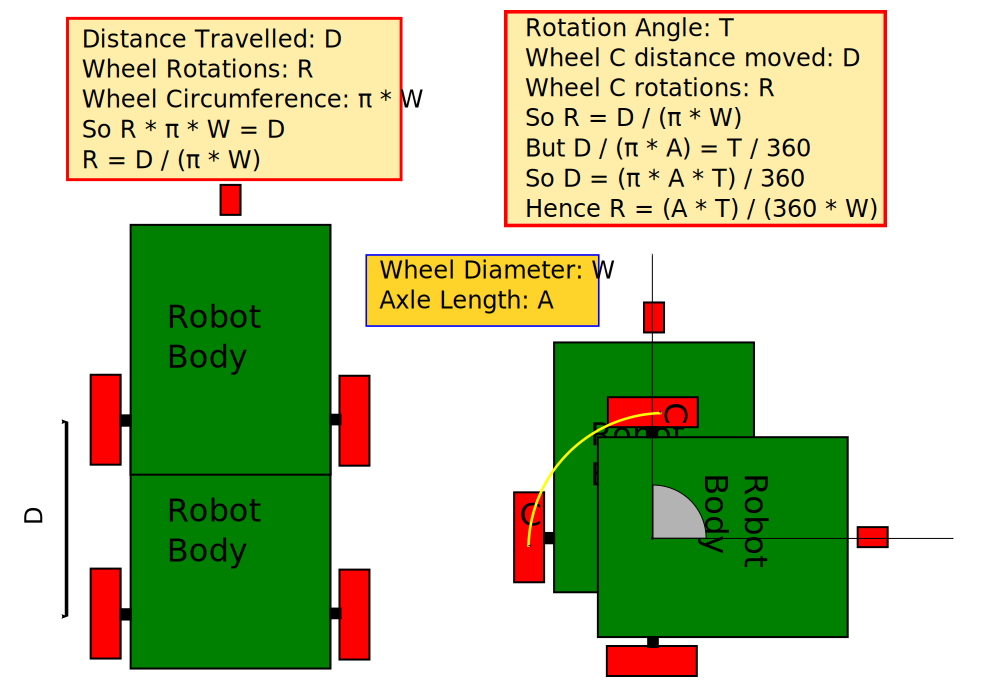
\includegraphics[width=0.7\textwidth]{Images/Pilot2}}
\note[item]{Please refresh your knowledge of plane geometry if you want to - but these equations are built into the Pilot}
\end{frame}

\begin{frame}
\frametitle{Pilots are brilliant}
\begin{block}{Pilots do the maths and run the threads - use them to mediate}
\begin{itemize}
 \item A \lstinline!MovePilot! object controls two motors at once.
 \item \textcolor{violet}{Internally it creates threads which watch the motors.}
 \item \textcolor{OliveGreen}{So it can start two motors rotating at the same time!}
 \item \textcolor{teal}{Easier and better than you synchronising them.}
\end{itemize}

\end{block}

\begin{block}{Cars and Pilots}
 \begin{itemize}
  \item Of course, a \lstinline!MovePilot! does not correspond to a real world object.
  \item \textcolor{OliveGreen}{It mediates between your program and a pair of wheels.}
  \item \textcolor{purple}{It provides simple methods like \lstinline!travel!, \lstinline!rotate! and \lstinline!arc!.}
\item The \lstinline!MovePilot! (differential) needs to know the wheel positions.
\item These positions are stored in a \lstinline!WheeledChassis! passed to the  \lstinline!MovePilot!. 
 \end{itemize}
\end{block}

\end{frame}

% \subsection*{Examples}
\begin{frame}[fragile]{Pilot Square}
\note[item]{Apart from construction, Pilots are incredibly simple to use!}
\note[item]{Do the magic numbers offend you.  Would you use side (or i- URGGH) in the loop}
\begin{lstlisting}[basicstyle=\ttfamily\scriptsize\color{blue},emph={MovePilot, pilot, ws,WheeledChassis,Wheel,ModelWheel, offset}]
public class SquarePilot {
 public static void main(String [] args) {
  // Wheel Diameter 60mm, both wheels set 29mm from car centre
  BaseRegulatedMotor mL = new EV3LargeRegulatedMotor(MotorPort.A);
  Wheel wL = WheeledChassis.modelWheel(mL, 60).offset(-29); 

  BaseRegulatedMotor mR = new EV3LargeRegulatedMotor(MotorPort.D);
  Wheel wR = WheeledChassis.modelWheel(mR, 60).offset(29);
  Wheel[] wheels = new Wheel[] {wR, wL};
  Chassis chassis = new WheeledChassis(wheels, WheeledChassis.TYPE DIFFERENTIAL);
  MovePilot pilot = new MovePilot(chassis);
  for (int side = 0 ; side < 4 ; side++) {
    pilot.travel(300);
    pilot.rotate(90);
  }
 }
}

\end{lstlisting}
\end{frame}

\begin{frame}{A Pose Provider}
\begin{block}{Odometry}
\begin{itemize}
\item A \lstinline!PoseProvider! is an object that tells you the current pose of the robot.
\item It could:
\begin{itemize}
  \item Watch the \lstinline!Pilot! and update its position when a move finishes (\textcolor{purple}{Odometry}).
  \item Ignore the \lstinline!Pilot! and use \textcolor{OliveGreen}{GPS},
  \item Use odometry and also update when it sees \textcolor{OrangeRed}{Landmarks using a Camera},
  \item Use the \textcolor{violet}{distances from the walls, and a map}, to work out where it is,
  \item Use \textcolor{BrickRed}{a BlueTooth connection to a human} to tell it where it is.
\end{itemize}
\item \textcolor{teal}{It could even combine a collection of methods to get the most reliable pose.}
\item \textcolor{RedOrange}{It is quite tempting to write your own \lstinline!PoseProvider!}
\end{itemize}
\end{block}
\end{frame}


\begin{frame}{The Odometry Pose Provider}
\begin{block}{Some EV3Dev Objects useful for navigation}
\begin{itemize}
\item We use a \lstinline!Pilot! to control the motors.
\item The \lstinline!Pilot! that we use for two driven motors is a \lstinline!MovePilot!.
\item \textcolor{RedOrange}{If you have some other movement system then you may need to write your own \lstinline!Pilot!.}
\item We also use a \lstinline!PoseProvider! to find out where we are.
\item The simple \lstinline!OdometryPoseProvider! pose provider (in leJOS) uses odometry.
\item \textcolor{RedOrange}{It is tempting to extend the \lstinline!OdometryPoseProvider! class to make it better.}
\end{itemize}
\end{block}
\end{frame}

\begin{frame}[fragile]{Odometry Example}
\begin{lstlisting}[emph={poseP, pilot},linewidth=14cm,basicstyle=\ttfamily\scriptsize\color{blue}]
public class WhereAmI {
 public static void main(String[] args) throws Exception {
  // Wheel Diameter 60mm, both wheels set 29mm from car centre
  BaseRegulatedMotor mL = new EV3LargeRegulatedMotor(MotorPort.A);
  Wheel wL = WheeledChassis.modelWheel(mL, 60).offset(-29); 
  BaseRegulatedMotor mR = new EV3LargeRegulatedMotor(MotorPort.D);
  Wheel wR = WheeledChassis.modelWheel(mR, 60).offset(29);
  Wheel[] ws = new Wheel[] {wR, wL};
  Chassis chassis = new WheeledChassis(wheels, WheeledChassis.TYPE DIFFERENTIAL);
  MovePilot pilot = new MovePilot(chassis);
  PoseProvider poseP = new OdometryPoseProvider(pilot);
  for (int side = 0 ; side < 4 ; side++) {
   pilot.travel(300); pilot.rotate(90);
  }
  LCD.drawString(0,0,poseP.getPose().toString());
  Button.Enter.waitForPressAndRelease();
 }  
}
\end{lstlisting}
\end{frame}

\begin{frame}{Tips and Tricks}
\begin{block}{Posing Problems - robots need to cheat}
\begin{itemize}
  \item \alert{Do not rely on odometry}
  \item \textcolor{OliveGreen}{Use touch sensors at the end of tracks}
  \item \textcolor{OliveGreen}{Use marks on a track and a light sensor}
  \item \textcolor{OliveGreen}{Use gears (fixed in a cage) and a geared track}
  \item \textcolor{OliveGreen}{Use accurate distance sensors}
\end{itemize}
\end{block}
\end{frame}


\begin{frame}{A Robot with a Pilot and a watching Thread}
\begin{center}
\href{https://youtu.be/yYER8YDCU2c}{\XeTeXLinkBox{\includegraphics[width=8cm,height=4.5cm]{Videos/MyCar.png}}}
\end{center}

\begin{block}{You will be programming this behaviour}
Except that this robot has rack and pinion (not differential) steering .
\end{block}
\end{frame}


\section*{Navigation in leJOS\\Waypoints, Poses, Maps and Paths.}

\begin{frame}{Finding your way around the leJOS way}
\begin{block}{Poses, Waypoints and Paths}
\begin{itemize}
  \item The leJOS world is defined by coordinates.
  \item Directions are relative to the x-axis.
  \item Rotation anti-clockwise increases the angle, so the y-axis is 90\degree.
  \item A \lstinline!Pose! is the position and orientation of the robot.
  \item When a robot program begins its pose is  $\left<(0,0), 0\degree\right>$.
  \item A \lstinline!Waypoint! is a position on the map.
  \item A \lstinline!Path! is a list of \lstinline!Waypoint! objects.
\end{itemize}
\end{block}
\end{frame}

\begin{frame}[plain]
  \begin{tikzpicture}[remember picture,overlay]
    \node[at=(current page.center)] {
      \includegraphics[height=\paperheight]{../Handouts/navigation.png}
    };
  \end{tikzpicture}
\end{frame}

%\subsection{leJOS Navigation}

\begin{frame}{The Navigator}
\note[item]{A question in the quiz asks why more waypoints might be better - the answer is on this slide}
\begin{block}{Some more leJOS Objects for navigation}
\begin{itemize}
\item We use a \lstinline!Navigator! to navigate a path.
\item It sends a \lstinline!Pilot! commands to move along a \lstinline!Path!
\item \textcolor{OliveGreen}{It also  checks after at each \lstinline!Waypoint! that it is on course using a \lstinline!PoseProvider!.}
\item There is a simple \lstinline!Navigator! class in leJOS that we can use.
\item The \lstinline!Navigator! constructor takes a \lstinline!PoseProvider! object and a \lstinline!Pilot!.
\item Call \lstinline!followPath! in your \lstinline!Navigator! to begin the path.
\end{itemize}
\end{block}
\end{frame}

\begin{frame}[fragile]{Example Navigation using a set of known waypoints}
\note[item]{Pause and have a good look at this correct way of navigating a square}
\note[item]{Notice that followPath is non-blocking.  So we have to wait for the path to finish afterwards}
\vspace*{-3mm}
\begin{lstlisting}[emph={Navigator, nav, Waypoint, Path}, basicstyle=\ttfamily\scriptsize\color{blue}]
public class PathFollowing {
 public static void main(String[] args) throws Exception {
  BaseRegulatedMotor mL = new EV3LargeRegulatedMotor(MotorPort.A);
  Wheel wL = WheeledChassis.modelWheel(mL, 60).offset(-29); 
  BaseRegulatedMotor mR = new EV3LargeRegulatedMotor(MotorPort.D);
  Wheel wR = WheeledChassis.modelWheel(mR, 60).offset(29);
  Wheel[] wheels = new Wheel[] {wR, wL};
  Chassis chassis = new WheeledChassis(wheels, WheeledChassis.TYPE DIFFERENTIAL);
  MovePilot pilot = new MovePilot(chassis);

  PoseProvider poseP = new OdometryPoseProvider(pilot);
  Navigator navigator = new Navigator(pilot, poseP);
  Path route = new Path();
  route.add(new Waypoint(100,0)); route.add(new Waypoint(100,100));
  route.add(new Waypoint(0,100)); route.add(new Waypoint(0,0));
  navigator.followPath(route); // followPath returns immediately, so
  navigator.waitForStop(); // we wait for the Navigator to stop!
 }
}
\end{lstlisting}
\end{frame}

\begin{frame}{Stopping a path to do something else}
\begin{block}{We can stop a \Verb!Navigator! in another \Verb!Thread! and resume it later.}
\begin{itemize}
\item We can use a \lstinline!Thread! to watch a sensor.
\item Then we can stop a \lstinline!Navigator! in the watching \lstinline!Thread!.
\item In the main thread we can wait until its safe to resume following the \lstinline!Path!.
\end{itemize}
\end{block}
\end{frame}

\begin{frame}[fragile]{Example Navigation}
\note[item]{Both the simplest and the cleverest way to go around a square - watching for obstacles}
\vspace*{-3mm}
\begin{lstlisting}[basicstyle=\ttfamily\tiny\color{blue}]
public class PathFinding {
  public static void main(String[] args) throws Exception {
    float[] samples = new float[1]; // Updated with the distances.
    // Create Navigator (nav), Path (route) as usual.
    .....
    Thread t = new Watcher(nav, samples); t.start();
    nav.followPath(route); nav.waitForStop(); // The read ahead paradigm again
    while (!nav.pathCompleted()) {
      while (samples[0] < 0.25f) { // Start again when obstacle > 25cm
        Sound.beep(); Delay.msDelay(500); 
      }
      nav.followPath(); nav.waitForStop();
    }
  }
}
public class Watcher extends Thread {
  private Navigator nav; private float[] dist;
  public Watcher(Navigator _nav, float[] _s) { nav = _nav; dist = _s;}
  public void run() {
    EV3UltrasonicSensor us = new EV3UltraSonicSensor(SensorPort.S1);
    SampleProvider sp = us.getDistanceMode();
    while (true) {
      sp.fetchSample(dist, 0);  // Fetch the distance into the shared samples array every time around this loop.
      if (dist[0] < 0.10f && nav.isMoving()) { nav.stop(); } // Obstacle!
    }
  }
}
\end{lstlisting}
\end{frame}

\begin{frame}{Maps}
\note[item]{If you draw an obstacle on a map as a square the path finder will happily plan a path through the corners of the square}
\begin{block}{A Map in leJOS is a set of lines - used to keep a robot away from danger}
\begin{itemize}
\item We use a \lstinline!LineMap! to tell the robot where things are in its environment.
\item A \lstinline!LineMap! object has a list of lines and a rectangular bounding box.
\item We use the \lstinline!Line! objects to mark out obstacles.
\item We use a \lstinline!PathFinder! to build a \lstinline!Path! through a \lstinline!LineMap!
\item The \lstinline!PathFinder! will not go outside the boundary, nor cross any \lstinline!Line!.
\item We tell the \lstinline!PathFinder! the starting \lstinline!Pose! and an ending \lstinline!Waypoint!.
\item The \lstinline!ShortestPathFinder! uses a clever algorithm to find the shortest path.
\item \textbf{A \lstinline!PathFinder! will never cross a line in the map.}
\item \textbf{A \lstinline!PathFinder! is happy to go through the end of a line.}
\end{itemize}
\end{block}
\end{frame}

\begin{frame}[fragile]{Getting there quickly}
\note[item]{If you think about it is amazing that this is such a short program}
\begin{lstlisting}[emph={bounds, myMap, pf, route, nav}, basicstyle=\ttfamily\scriptsize\color{blue}]
public class PathFinding {
 public static void main(String[] args) throws Exception {
  // Create Navigator (nav) as usual.
  .....

  Line [] lines = new Line[4];
  lines [0] = new Line(-20f, 20f, 100f, 20f);
  lines [1] = new Line(-20f, 40f, 20f, 40f);
  lines [2] = new Line(-20f, 60f, 20f, 60f);
  lines [3] = new Line(-20f, 80f, 20f, 80f);
  Rectangle bounds = new Rectangle(-50, -50, 250, 250);
  LineMap myMap = new LineMap(lines, bounds);
  PathFinder pf = new ShortestPathFinder(myMap);
  Path route = pf.findRoute(new Pose(0,0,0), new Waypoint(0, 100));
  nav.followPath(route);
  nav.waitForStop();
 }
}
\end{lstlisting}
\end{frame}

%%%%%%%%%%%%%%%%%%%%%%%%%%%%%%%%%%%%%%%%%%%%%%%%%%%%%%%%%%%%%%%%%%%%%%%%%%%%%%%%%%%%%%%%%%%

\lecture{Behaviours, Project Extras and Grading}{LectureFive}


\begin{frame}<handout:0>{First - more about good programming!}
\note[item]{Taling about grading - remember that you will be judged in the end on how much contribution you made to the project.  This is not just coding, but it is mostly coding.}

\begin{center}
\includegraphics[height=6cm]{Images/pisa.jpg}
\end{center}
\note[item]{Many people see nothing wrong with this building (apparently)}
\end{frame}

\begin{frame}[fragile]{Feedback}
\begin{lstlisting}
int x; boolean t; x = 0; // WTF
for (x = 1; x <= 5; x = x + 1){mLeft.forward();
Delay.msDelay(173);} // WTF (three or four times)
NXTSoundSensor ss = new NXTSoundSensor(SensorPort.S3);
SampleProvider sp = ss.getDBAMode();
float[] samples = new float[1];
ss.fetchSample(samples, 0); 
if (samples[0] > 0.50f) { // For Nuno!
  return(true);
else {
  return (false);
} // BIG WTF
\end{lstlisting}
\note[item]{There is so much wrong with this (working) code.}
\note[item]{x, t are not variable names}
\note[item]{x=1, x<=5 is not the paradigm}
\note[item]{What about nice formating}
\note[item]{173 is a magic number}
\note[item]{Nice to see a float literal rather than the double 0.50}
\note[item]{Do not use many lines when one line is better - do not use one where many are better!}
\note[item]{return is not a function - so no brackets please.}
\end{frame}
\begin{frame}[fragile]{Feedback}
\begin{lstlisting}
final int FORWARD_TIME = 173;
final int SIDES = 4;

for (int side = 0; side < SIDES; side++){
   mLeft.forward();
   Thread.sleep(FORWARD_TIME);
}
NXTSoundSensor ss = new NXTSoundSensor(SensorPort.S3);
SampleProvider sp = ss.getDBAMode();
float[] samples = new float[1];
ss.fetchSample(samples, 0); 
return samples[0] > 0.50f;
\end{lstlisting}
\end{frame}

\begin{frame}[fragile]{Its Final}
\begin{block}{Naming Numbers}
\begin{itemize}
\item Its \textcolor{purple}{nice} to use words instead of having to type numbers.
\item We \alert{should} use \lstinline!Math.PI! instead of remembering 3.141592654...
\item \textcolor{OliveGreen}{Its better to use a name that you define once (like \lstinline!WHEEL_SIZE!).}
\item When you change the wheels, you only have to change one line of code.
\item \textcolor{OliveGreen}{Define constants just like other fields, but in UPPER CASE.}
\item Use \textcolor{violet}{Comments} to help the reader (you in a week).
\item \textbf{Do not use static (global) objects!}\\
\textcolor{BrickRed}{Create them in a short \lstinline!main!\\}
\textcolor{teal}{Pass objects to the constructor of other classes.}
\note[item]{The last part about global objects is a mantra of mine.}
\note[item]{It is okay to have public final static constants.  It is NOT fine to have public objects ever. WORK OF THE DEVIL}
\note[item]{Sometimes - for the sake of space - I have been forced to do this on slides - You Must Not}
\end{itemize}
\end{block}
\end{frame}

\section{Behaviours\\ The Rodney Brooks subsumption architecture}
\note{Rodney Brooks led a pioneering team in MIT in 1986 who introduced this framework}
\begin{frame}
\begin{block}{We have to manage complex robot behaviour}
\begin{itemize}
    \item \textcolor{teal}{We managed robot movement using the navigation stack}
    \item \textcolor{BrickRed}{Now we need to combine many simple tasks}
    \item \textcolor{OliveGreen}{To make a robot that appears intelligent}
    \item \textcolor{OliveGreen}{To make a robot that plans to achieve its goals}
    \item \textcolor{purple}{Better than Threads: Who's watching that Battery Voltage?}
\end{itemize}
\end{block}
\end{frame}

\begin{frame}{Subsumption}
\begin{block}{A guy with three active \textcolor{yellow}{behaviours}}
\begin{itemize}
\item walking along (\textcolor{OliveGreen}{behaviour 1}),
\item eating (\textcolor{purple}{behaviour 2}) and
\item chatting (\textcolor{teal}{behaviour 3}).
\item \dots who falls over - arms shoot forwards (\textcolor{teal}{behavior 4} \textcolor{BrickRed}{subsumption}).
\end{itemize}

\alert{It is vitally important that behaviours subsume each other.}
\end{block}
\end{frame}

\begin{frame}[fragile]{Subsumption architecture}

\begin{columns}
\begin{column}{0.6\textwidth}
\begin{block}{Plants \textcolor{yellow}{do not} grow towards the sun.}
\begin{itemize}
\item \textcolor{OliveGreen}{The hormone Auxin promotes growth.}
\item \textcolor{BrickRed}{The hormone Auxin is denatured by sunlight.}
\item \textcolor{teal}{Plants have no intelligence (Charles).}
\item \alert{Behaviours} just get triggered.  
\item \textcolor{purple}{Plant cells grow when not in sunlight.}
\item \textbf{Responsive behaviours = Complexity.}
\end{itemize}
\end{block}
\end{column}
\begin{column}{0.4\textwidth}
\begin{center}
\href{http://plantsinmotion.bio.indiana.edu/plantmotion/MovieFiles/CornSunWorship.m4v}{\XeTeXLinkBox{\includegraphics[width=5cm,height=3.5cm]{Videos/corn.png}}}
\end{center}
\end{column}
\end{columns}
\end{frame}

\begin{frame}{Subsumption}
\begin{block}{A Group of behaviours is  \textcolor{yellow}{intelligence}}
\begin{itemize}
\item \alert{No central controller}.
\item Behaviours have \alert{conditions} on which they become active.
\item Behaviours control different \alert{activities}.
\item When \alert{active} they do their thing.
\item They are \alert{suppressed} by \alert{higher level} behaviours.
\end{itemize}

\textcolor{OliveGreen}{\textbf{Do you remember the last time \emph{conditions} made you touch your face/hair.}}
\end{block}
\note{It is thought that well over 90\% of all that we do is sub-conscious - read behaviour driven.}
\end{frame}

\begin{frame}[fragile]{The Behaviour Stack: Subsumption in leJOS}
\begin{block}{An \lstinline[identifierstyle=\bfseries\color{yellow}]{Arbitrator} manages a list of \lstinline[identifierstyle=\bfseries\color{yellow}]!Behavior! objects.}
\begin{itemize}
\item \textcolor{BrickRed}{Loops forever} asking each \lstinline!Behavior! object whether it wants to \lstinline!takeControl!.
\item \textcolor{OliveGreen}{Runs the highest priority \lstinline!action! method} in its own thread.
\end{itemize}
\end{block}

\begin{lstlisting}[emph={Behavior,suppress,takeControl,action}]
WHILE TRUE:
  // Build a list of waiting Behaviour actions
   ASK each Behavior if it wants to takeControl.

   IF no Behavior action is currently running THEN:
      RUN highest priority waiting Behavior
   ELSE IF there is a higher priority Behavior waiting
      // Notice that we NEVER STOP a currently active Behaviour
      CALL suppress on the currently running Behavior

\end{lstlisting}
\note{Just saying loops forever does not mean it keeps looping FAST - sometimes a statement in the loop blocks! - slowing the loop down}
\end{frame}

\begin{frame}{The Behaviour Stack: Subsumption in leJOS}
\begin{block}{Subsumption - \lstinline[identifierstyle=\bfseries\color{yellow}]!suppress! and \lstinline[identifierstyle=\bfseries\color{yellow}]!action! run in different Threads}
\begin{itemize}
\item CASE ONE: \textcolor{BrickRed}{When a \lstinline!Behavior! is running\\}
 \textcolor{OrangeRed}{and a higher priority \lstinline!Behavior! needs to take over}

\dots \textcolor{teal}{the \lstinline!Arbitrator! keeps calling \lstinline!suppress!\\}
\dots \textcolor{OliveGreen}{eventually this running \lstinline!Behaviour! will get the message (and stop)}
\item CASE TWO: \textcolor{BrickRed}{When no \lstinline!Behavior! is currently running}

\dots \textcolor{teal}{the \lstinline!Arbitrator! starts the highest priority waiting \lstinline!Behavior!}
\end{itemize}
\note[item]{You have a part of the Arbitrator that runs the action methods, and another part (in another thread) that is running suppress and takecontrol}
\note[item]{One Behaviour can be running two methods (sharing the bahaviour state - in two different thread)}
\note[item]{Patting your tummy and stroking your head.}
\note[item]{SOmeone knocking on the door (suppress) when you are very busy doing something (action)}
\end{block}
\begin{block}{The \lstinline[identifierstyle=\bfseries\color{yellow}]!suppress! method can be called any number of times (including none).}
\begin{itemize}
\item If a \lstinline!Behavior! has a short \lstinline!action! then it can ignore \lstinline!suppress! calls.\\
\textcolor{OliveGreen}{The \lstinline!action! will finish in good time anyway.}
\item A long running \lstinline!action! method must notice \lstinline!suppress!.\\ 
\textcolor{OliveGreen}{The \lstinline!action! method should finish early and exit gracefully.}
\end{itemize}

\end{block}
\end{frame}

\begin{frame}[fragile]{Subsumption in leJOS: The \lstinline!Behavior! interface}
\begin{block}{An \lstinline[identifierstyle=\bfseries\color{yellow}]!Arbitrator! manages a list of \lstinline[identifierstyle=\bfseries\color{yellow}]!Behavior! objects.}
Every \lstinline!Behavior! in leJOS must implement these three methods
\begin{itemize}
\item a \lstinline!boolean takeControl()! that the \lstinline!Arbitrator! calls to see if it wants control.
\item an \lstinline!void action()! that it wants to do when it has control.
\item a \lstinline!void suppress()! method the \lstinline!Arbitrator! invokes to persuade the \lstinline!Behavior! to finish quickly and exit gracefully.
\end{itemize}
\end{block}
\end{frame}

\begin{frame}{Understanding a \lstinline!Behavior!}
\begin{block}{A Single \lstinline[identifierstyle=\bfseries\color{yellow}]!Behavior! responds to a certain set of conditions}
\begin{itemize}
    \item \textcolor{BrickRed}{It deals with some problem} (e.g. Battery Voltage)
    \item \textcolor{OliveGreen}{It just gets some appropriate task done} (e.g. Turning Left, Going Home)
\end{itemize}
\end{block}

\begin{block}{leJOS lets us create many \lstinline[identifierstyle=\bfseries\color{yellow}]!Behavior! objects and think about them separately}
\begin{itemize}
\item  We let an \lstinline!Arbitrator! object organise them for us.
\item Each \lstinline!Behavior! takes control of the robot when it is active.
\item It \textbf{should} respond nicely when the \lstinline!Arbitrator! tells it to stop\ldots 
\item \ldots because another (more important) \lstinline!Behavior! needs a turn.
\end{itemize}
\end{block}
\end{frame}

\begin{frame}{Building a \lstinline!Behavior!}
\note[item]{I said that I would come back to this!}
\begin{block}{Sharing is playing nicely}
\begin{itemize}
\item We have a \alert{class} for each type of \lstinline!Behavior! that we need.
\item A \lstinline!Behavior! class may need access to the \lstinline!Pilot!, or the \lstinline!Navigator! or to \alert{sensors}.
\item A \lstinline!Behavior! class may need to access some \alert{state control object}.
\item It is fine to store the (shared) objects as local variables in your \lstinline!main! method.
\item Pass each (shared) object (as needed) into the constructor for a \lstinline!Behavior! object.
\item Each \lstinline!Behavior! object stores (a reference to) the shared object in a \lstinline!private static! field.
\item If only one \lstinline!Behavior! needs to access an object then push the object down to a (\lstinline!private static!) field in that class.
\item \textcolor{violet}{Construct and store objects as close  as possible to where they are needed.}
\end{itemize}
\end{block}
\end{frame}

\begin{frame}[fragile]{An example - Behaviour controlled driving}
\note{Notice that Driver does create a sensor as the US sensor is ONLY used by backup!}
\begin{lstlisting}[basicstyle=\ttfamily\scriptsize\color{blue}, xleftmargin=0in, linewidth=14cm,emph={pilot, Behavior,Arbitrator,go}]
public class Driver {
  public static void main(String[] args) {
   MovePilot pilot = getPilot(MotorPort.A, MotorPort.B, 60, 29);
   pilot.setLinearSpeed(200);
   Behavior trundle = new Trundle(pilot);
   Behavior escape = new Escape(pilot);
   Arbitrator ab = new Arbitrator(new Behavior[] {trundle, escape});
   ab.go();  // This never returns! It is a blocking call.
  }
  private static MovePilot getPilot(Port left, Port right, int diam, int offset) {
   BaseRegulatedMotor mL = new EV3LargeRegulatedMotor(left);
   Wheel wL = WheeledChassis.modelWheel(mL, diam).offset(-1 * offset); 
   BaseRegulatedMotor mR = new EV3LargeRegulatedMotor(right);
   Wheel wR = WheeledChassis.modelWheel(mR, diam).offset(offset);
   Wheel[] wheels = new Wheel[] {wR, wL};
   Chassis chassis = new WheeledChassis(wheels, WheeledChassis.TYPE_DIFFERENTIAL);
   return new MovePilot(chassis);
  }
 }
 
\end{lstlisting}
\end{frame}
%
\begin{frame}[fragile]{An example \lstinline!Behavior! - Keep on Trucking}
\note{Lowest priority behaviour - only keep on trucking when you have nothing better to do}
\begin{lstlisting}[basicstyle=\ttfamily\scriptsize\color{blue}, xleftmargin=0in, linewidth=11cm,emph={pilot, private, Behavior,suppress,takeControl,action}]
public class Trundle implements Behavior {
  private MovePilot pilot;
  Trundle(MovePilot p) {
    this.pilot = p;  // Save the (shared) pilot in a field
  }
  // Start trundling and return control immediately.
  public void action() {
    pilot.forward();
  }
  // Since action returns immediately this is probably never called
  public void suppress() {}
  // Is it my turn?
  public boolean takeControl() {
    return true; // Yeah - we are SO eager
  }
}
\end{lstlisting}
\end{frame}

\begin{frame}[fragile]{An Example \lstinline!Behavior! - Get Me Out of Here}
\note{Here is that sensor in a private field}
\begin{lstlisting}[basicstyle=\ttfamily\scriptsize\color{blue}, xleftmargin=0in, linewidth=14cm,emph={Random, pilot, private, public class Backup, Behavior,suppress,takeControl,action}]
public class Escape implements Behavior {
  private MovePilot turner; // The passed in shared pilot
  private EV3UltrasonicSensor us = new EV3UltrasonicSensor(SensorPort.S1);
  private SampleProvider sp = us.getDistanceMode(); // This sensor will just be used by us
  private Random rgen = new Random(); // just used by us (a new piece of Java?)
  private float[] distance = new float[1]; // just used by us - clever name huh!
  Trundle(MovePilot p) {
    turner = p;
  }
  public void action() {
    turner.travel(-50);
    turner.rotate((2 * rgen.nextInt(2) - 1) * 30); // right or left 30 degrees at random.
  }
  public void suppress() { } // Not sensible to suppress this Behavior. Ignore suppress.
  public boolean takeControl() { // Is it my turn?
    sp.fetchSample(distance, 0);
    return (distance[0] < 0.20f);  // See how this is short, but still easy to read?
  }
}
\end{lstlisting}
\end{frame}

\section{Project Extras and more advanced programming}

\begin{frame}{State Based Behaviours}
\begin{block}{Your robot has to do one thing and then another}
\begin{itemize}
\item The conditions for a \lstinline!Behavior! may not just be sensors values
\item \textcolor{teal}{Think of a game where you alternate moves.}
\begin{itemize}
\item \textcolor{RedOrange}{A button press could disable all of my move behaviours.}
\item \textcolor{OliveGreen}{Another button press makes them possible again.}
\end{itemize}
\end{itemize}
\end{block}
\begin{block}{Use a shared \lstinline[identifierstyle=\bfseries\color{yellow}]!State! object to disable behaviours}
\begin{itemize}
\item \textcolor{teal}{(Only when \lstinline!state.getState() == 'M'!)}. Behaviours: \textcolor{OrangeRed}{Move to Thing}
\item \textcolor{teal}{(Only when \lstinline!state.getState() == 'P'!)}. Behaviours: \textcolor{Orange}{Pick up Thing}
\item \textcolor{teal}{(Only when \lstinline!state.getState() == 'I'!)}. Behaviours: \textcolor{OliveGreen}{Identify Thing}
\item \textcolor{teal}{(Only when \lstinline!state.getState() == 'H'!)}. Behaviours: \textcolor{violet}{Take Thing Home}
\end{itemize}
\end{block}
\end{frame}

\begin{frame}[fragile]{Sharing the \lstinline!State! object: What sort of state am I in?}
\begin{block}{State is a kind of internal sensor - looking at the \emph{state} of the robot}
\begin{itemize}
\item Create a \lstinline!State! class and then a \lstinline!State! instance \lstinline!state! in \lstinline!main!.
\item The \lstinline!state! will record what the robot is trying to do.
\item Share \lstinline!state! with any \lstinline!Behaviour! that depends on, or alters, the robot state.
\item The \lstinline!State! class can have a single \lstinline!char! field with getters and setters.
\end{itemize}
\end{block}
\begin{lstlisting}
public boolean takeControl() { // Check some condition
   return ... && state.getState == 'P'; //  AND it is our turn
}
public void action() { // Look for something
   ...
   state.setState(`I'); //  Got it! change to Identifying.
}
\end{lstlisting}
\end{frame}

\begin{frame}[fragile]{HARD: Using (shared) state for rising edge detection (separate claps)}
\note[item]{This robot is one of two states - waiting for a lull in sound betwen claps, and then waiting for a loud sound - which is the next clap}
\vspace*{-3mm}
\begin{lstlisting}[basicstyle=\ttfamily\scriptsize\color{blue}, xleftmargin=0in, linewidth=11cm,emph={State}]
public class State { // methods rather than a char field is better
  private boolean waitingForRising = true;
  public boolean isWaitingForRising() { return waitingForRising; }
  public void setWaitingForRising(boolean b) { waitingForRising = b; }
}
\end{lstlisting}
\vspace*{-3mm}
\begin{columns}[T]
\begin{column}{0.62\textwidth}
\begin{lstlisting}[basicstyle=\ttfamily\scriptsize\color{blue}, framexleftmargin=0.05in, xleftmargin=0in, linewidth=\textwidth,emph={takeControl, suppress, action, State}]
// wait for a loud sound after a quiet one
public class WFRise implements Behavior {
  private State sharedState;
  private float[] sound = new float[1];
  public boolean takeControl() {
    if (!sharedState.isWaitingForRising()) return false;
    sp.fetchSample(sound, 0);
    return (sound[0] > 0.5f);
  }
  public void suppress() {}
  public void action(){
    //  Do the "Heard a new clap" action
    sharedState.setWaitingForRising(false);
  } // constructor and sp def'n not shown
\end{lstlisting}
\end{column}
\begin{column}{0.45\textwidth}
\begin{lstlisting}[basicstyle=\ttfamily\scriptsize\color{blue}, framexleftmargin=0.0in, xleftmargin=-3mm, linewidth=1.04\textwidth,emph={takeControl, suppress, action, State}]
public class WFFall implements Behavior {
  private State sharedState;
  private float[] sound = new float[1];
  public boolean takeControl() {
    if (sharedState.isWaitingForRising()) {
      return false;
    }
    sp.fetchSample(sound, 0);
    return (sound[0] < 0.2f);
  }
  public void suppress() {}
  public void action() {
    sharedState.setWaitingForRising(true);
  } // constructor and sp def'n not shown
\end{lstlisting}
\end{column}
\end{columns}
\end{frame}


\begin{frame}{States and Personality}
\note{mention popes and parents}
\begin{block}{Changing from one state of certainty to another}
\begin{itemize}
\item \textcolor{OliveGreen}{We can control the flow of behaviours using a shared state.}
\item \alert{Drawing a state diagram is a very useful process.}
\item Groups of behaviours may be self-contained, e.g. behaviours for finding food.
\item A robot appears to have a certain \alert{personality} when doing these behaviours.
\item Of course, \textcolor{purple}{different personalities can share some behaviours.}
\item \textcolor{OliveGreen}{We can make a table of which behaviours are possible in each personality.}
\end{itemize}
\end{block}
\end{frame}


\begin{frame}{Worrying Pitfalls}

\begin{block}{\lstinline[identifierstyle=\bfseries\color{yellow}]!suppress! must make \lstinline[identifierstyle=\bfseries\color{yellow}]!action! stop}
\begin{itemize}
\item After calling an \lstinline!action! method no other \lstinline!action! can start until this one finishes.

\item Long running \lstinline!action! methods that ignore calls to \lstinline!suppress! break the system.

\item  \lstinline!suppress!  can set a field that is checked by \lstinline!action! method, causing it to return.
\end{itemize}
\end{block}
\begin{block}{Fast Methods}
\begin{itemize}
\item If \lstinline!action! never takes a long time then \lstinline!suppress! can just return.

\item \textcolor{BrickRed}{\lstinline!suppress! should always return quickly.}

\item \lstinline!suppress! will be called multiple times if \lstinline!action! takes a while to finish.
\end{itemize}
\end{block}
\end{frame}



\section*{Extra Sensors, Extra Programs}
\begin{frame}{Extra Sensors}
\begin{block}{The cyclingProfessor GitHub  account}
The Android app in the \href{https://github.com/cyclingProfessor/EV3Sensors}{EV3Sensors} repository, connects to a leJOS brick.

  It does \alert{OpenCV image processing}, \alert{continually finds QR codes} and \alert{reads NFC tags}.

The Readme.md in the repository tells you how to make this work.
\begin{itemize}
  \item You can use it as a set of extra sensors for your brick.
\end{itemize}
\end{block}

\begin{block}{The examples repository contains several interesting examples}
The \href{https://github.com/cyclingProfessor/LejosExamples}{LejosExamples} repository includes code for the leJOS end of EV3Sensors.  

\textbf{\textcolor{OliveGreen}{It also contains the (in progress) PCMapper program.}}
\end{block}
\end{frame}

\begin{frame}{QR, NFC, FaceFinder and Proximity Sensor}
\begin{block}{EV3Sensors app internals - \textcolor{yellow}{you do not NEED to know this to use QR codes}}
\begin{itemize}
\item  \lstinline!ChatFragment.sendMessage! sends a \lstinline!String! to the brick.
\item 
\lstinline!ChatFragment.mHandler.handleMessage! processes messages from the EV3 in the (switch) case \lstinline!MESSAGE_READ!.  
\item Messages from the EV3 are shown in a \lstinline!ListView!.
\item NFC tag and QR code data etc.,  are all be sent to the EV3 brick.
\item There is example OpenCV blob detection in the app.  
\item You can easily detect faces using openCV with the app.
\item Advanced: you can use all other phone sensors.
\end{itemize}
\end{block}
\end{frame}

\begin{frame}{The PCMapper}
\begin{block}{Using the PC as an \textcolor{yellow}{output} or \textcolor{yellow}{control} device or even a {\emph{\textcolor{yellow}{GPS} Sensor}}}
\begin{itemize}
\item Using EV3Sensors you can use your mobile phone to read QR codes etc.,
\item Your leJOS program can connect \textbf{at the same time} to a PC/laptop.
\item You can use this (PC) to display, for example, the robot position on a map.
\item You could use this as a way of updating an extended \lstinline!OdometryPoseProvider!.
\item Perhaps when you click the map, it sends an updated \lstinline!Pose! to the robot.
\item My example (PCMApper, EV3mapper) can be modified for your purposes.
\end{itemize}
\end{block}
\end{frame}


\begin{frame}{Self Test}
\begin{block}{Questions}
\begin{enumerate}
 \item Are you ready?
\end{enumerate}

\end{block}
\end{frame}

\end{document}
